\documentclass[10pt]{article}

% Math environment, symbols, bbm fonts, doublestroke fonts, physics for partial derivatives (pdv{}{}), breqn for multi-line equations
\usepackage{amsmath,amssymb,bbm,dsfont,physics,breqn}
% Define plim operator
\DeclareMathOperator*{\plim}{plim}
% Page size and margins
\usepackage{geometry}
\geometry{letterpaper,tmargin=1in,bmargin=1in,lmargin=1in,rmargin=1in}
% Line spacing
\usepackage{setspace}
\setstretch{1.5} % 1 for default line spacing, 2 for double, etc.
% Hyperlink environment
\usepackage{hyperref}
\hypersetup{colorlinks,linkcolor=red,urlcolor=blue,citecolor=red}
% Table environment
\usepackage{booktabs}
% Threeparttable environment
\usepackage[flushleft]{threeparttable}
% Graphic environment
\usepackage{graphicx}
% Subfigures
\usepackage{subcaption}
% Allows float options (e.g. [H] or [!ht])
\usepackage[capposition=top]{floatrow}
% Indents first paragraph
\usepackage{indentfirst}
% Footnotes go to bottom of page
\usepackage[bottom]{footmisc}
% Bibliography with AER style
\usepackage{natbib}
\bibliographystyle{aer}

% Custom section/subsection formatting
\usepackage{titlesec}
% Make section be arabic
\renewcommand{\thesection}{\arabic{section}}
% Make subsection be arabic
\renewcommand{\thesubsection}{\thesection.\arabic{subsection}}
% Make subsubsections be arabic
\renewcommand{\thesubsubsection}{\thesubsection.\arabic{subsubsection}}
% Section title formatting
\titleformat{\section}%
   {\flushleft\bfseries\LARGE}{\thesection}{0.5em}{}
% Subsection title formatting
\titleformat{\subsection}%
   {\Large\bfseries}{\thesubsection}{0.5em}{}
% Subsubsection title formatting
\titleformat{\subsubsection}%
          {\large\bfseries}{\thesubsubsection}{0.5em}{}
% Paragraph title formatting
\setcounter{secnumdepth}{4}
\titleformat{\paragraph}%
          {\large\bfseries}{\theparagraph \newline}{0.5em}{}
% Bibliography title formatting
% Bibliography doesn't using \section*
\renewcommand{\bibsection}{%
   \newpage
   \flushleft{\LARGE{\textbf{{\refname}%
   }}}
}
% Appendix autoref
\usepackage{appendix}
\newcommand{\aref}[1]{\hyperref[#1]{Appendix~\ref{#1}}}

% Automatically label sections
\usepackage{letltxmacro}
\LetLtxMacro{\oldsection}{\section}
\renewcommand{\section}[2][]{\oldsection[#1]{#2}\index{#1}\label{sec:\thesection}}
\LetLtxMacro{\oldsubsection}{\subsection}
\renewcommand{\subsection}[2][]{\oldsubsection[#1]{#2}\index{#1}\label{sec:\thesubsection}}
\LetLtxMacro{\oldsubsubsection}{\subsubsection}
\renewcommand{\subsubsection}[2][]{\oldsubsubsection[#1]{#2}\index{#1}\label{sec:\thesubsubsection}}

% autoref prints sections/subsections as Section
\renewcommand{\sectionautorefname}{Section}
\renewcommand{\subsectionautorefname}{Section}
\renewcommand{\subsubsectionautorefname}{Section}

% Custom page numbering
\usepackage{fancyhdr,lastpage}
\pagestyle{fancy}
\lfoot{\footnotesize\textsl{\hyperref[sec:1]{Introduction} - \hyperref[sec:2]{Data} - \hyperref[sec:3]{Model} - \hyperref[sec:4]{Results} - \hyperref[sec:5]{Conclusion} - \hyperref[sec:A]{Appendix}}}
\rfoot{\footnotesize\textsl{Page \thepage\ of \pageref{LastPage}}}
\lhead{} % Remove filler
\chead{} % Remove filler
\rhead{} % Remove filler
\cfoot{} % Remove default page number
\renewcommand\headrulewidth{0pt} % Remove top line

% Equations numbered by section/subsection
\numberwithin{equation}{subsection}
% No more . inside of equation tags, instead say eqn.
\renewcommand{\theequation}{\thesubsection \text{ eqn.} \arabic{equation}}

% Suppress underfull \hbox warning
\hbadness=10000

% Custom enumerate
\renewcommand{\theenumi}{\alph{enumi}}

% Result dir
\newcommand*{\FigureDir}{../../graphs}
\newcommand*{\DemoDir}{../../code/Rick/OUTPUT/Demographics}
\newcommand*{\SSDir}{../../code/Rick/OUTPUT/SS}
\newcommand*{\TPDir}{../../code/Rick/OUTPUT/TP}

% Colors
\usepackage{xcolor}
\newcommand{\red}{\color{red}}
\newcommand{\blue}{\color{blue}}

\begin{document}

% %%%%%%%%%%%%%%%%%%%%%%%%%%%%%%%%%%%%%%%%%%%%%%%%%
% \section{EXAMPLE USAGE OF FIGURE AND TABLE}
% %%%%%%%%%%%%%%%%%%%%%%%%%%%%%%%%%%%%%%%%%%%%%%%%%

% FIGURES

% \begin{figure}[H]
%    \centering
%    \caption{\label{fig:p\thesubsection}\autoref{sec:p\thesubsection}}
%    \scalebox{1}{
%       \begin{threeparttable}
%          \begin{tabular}{cc}
%             \includegraphics[width=0.50\textwidth]{\FigureDir/} &
%             \includegraphics[width=0.50\textwidth]{\FigureDir/} \\
%             \includegraphics[width=0.50\textwidth]{\FigureDir/} &
%             \includegraphics[width=0.50\textwidth]{\FigureDir/}
%          \end{tabular}
%       \end{threeparttable}
%    }
% \end{figure}

% SIDE BY SIDE FIGURES WITH CAPTIONS

% \begin{figure}[H]
%    \caption{\label{fig:\thesubsubsection.1}}
%    \begin{subfigure}{0.5\textwidth}
%       \centering
%       \includegraphics[width=\textwidth]{\SSDir/static/images/SS_n.png}
%       \caption{Subfig 1}
%    \end{subfigure}% <-- this "%" symbol is important
%    ~ % <-- this "~" symbol is important
%    \begin{subfigure}{0.5\textwidth}
%       \centering
%       \includegraphics[width=\textwidth]{\SSDir/dynamic_partial/images/SS_n.png}
%       \caption{Subfig 2}
%    \end{subfigure}
%    \newline <-- this creates a new lines
%    \begin{subfigure}{0.5\textwidth}
%       \centering
%       \includegraphics[width=\textwidth]{\SSDir/dynamic_full/images/SS_n.png}
%       \caption{Subfig 3}
%    \end{subfigure}%
%    ~ % <-- this "~" symbol is important
%    \begin{subfigure}{0.5\textwidth}
%       \centering
%       \includegraphics[width=\textwidth]{\SSDir/dynamic_full/images/SS_n.png}
%       \caption{Subfig 4}
%    \end{subfigure}
% \end{figure}

% TABLES

% \begin{table}[H]
%    \centering
%    \scalebox{0.75}{
%       \begin{threeparttable}\caption{\label{tab:p\thesubsection}\autoref{sec:p\thesubsection}}
%          \begin{tabular}{lcc}
%             \hline\hline\addlinespace
%             \input{../regression_tables/p1a.tex}
%             \addlinespace\hline\hline
%          \end{tabular}
%          \begin{tablenotes}
%             \item 
%             Standard errors in parentheses.
%          \end{tablenotes}
%       \end{threeparttable}
%    }
% \end{table}

% SIDE BY SIDE TABLES

% \begin{table}[H]
%    \begin{minipage}[t]{0.5\textwidth}
%      PUT TABLE 1 HERE
%    \end{minipage}% <-- this "%" symbol is important
%    \begin{minipage}[t]{0.5\textwidth}
%      PUT TABLE 2 HERE
%    \end{minipage}
% \end{table}

% How to reference sections: \autoref{sec:1}
% How to reference subsections: \autoref{sec:p1a}
% How to reference equations: \ref{eq:1a1} for section 1, subsection a, equation 1

% %%%%%%%%%%%%%%%%%%%%%%%%%%%%%%%%%%%%%%%%%%%%%%%%%
% \section{Thesis}
% %%%%%%%%%%%%%%%%%%%%%%%%%%%%%%%%%%%%%%%%%%%%%%%%%

% %%%%%%%%%%%%%%%%%%%%%%%%%%%%%%%%%%%%%%%%%%%%%%%%%
% \section{Title Page}
% %%%%%%%%%%%%%%%%%%%%%%%%%%%%%%%%%%%%%%%%%%%%%%%%%

\begin{titlepage}
\title{Estimation Effects of Various Demographic Forecasting Techniques in Japan Using an Overlapping Generations Model
         \thanks{I would like to thank Dr. Richard Evans for the guidance and support he provided while writing my thesis.}
      }
\author{
   Adam Alexander Oppenheimer
   \footnote{University of Chicago,
      Department of Economics. Email:
      \href{mailto:oppenheimer@uchicago.edu}
      {oppenheimer@uchicago.edu}.
   }
}
\date{May 2020 \\
   \scriptsize{}}
\maketitle
\vspace{-9mm}
\begin{abstract}
\small{The future of Japan will largely be shaped by its aging population. Many papers have estimated the macroeconomic effects of population aging through the use of forecasted demographics. However, are these results being unduly influenced by how demographics are being forecasted?
\par This paper attempts to shed light on the question of how various demographic forecasting techniques influence macroeconomic models of Japan. We consider four demographic models: the first (baseline) assumes constant demographics; the second assumes constant fertility, mortality, and immigration rates that describe an evolution of population; and the third and fourth use parametric and non-parametric models, respectively, to forecast fertility, mortality, and immigration rates over time that describe an evolution of population.
\par Our results indicate that demographic forecasting technique may have some influence on macroeconomic aggregate estimates. Unsurprisingly, the baseline model results differ markedly from the models that include population evolution over time. Among the models that include population evolution, transition path results, other than investment, appear to be largely unaffected by forecasting technique. However, steady state results may be greatly influenced by forecasting method used. Depending on the model used, concerns about population aging in Japan may be far worse than anticipated in previous research.

\vspace{3mm}

\noindent\textit{keywords:}\:
   Overlapping Generations Model,
   Demographic Transition,
   Japan Calibration

\vspace{3mm}

}

\end{abstract}
\thispagestyle{empty}
\end{titlepage}

% %%%%%%%%%%%%%%%%%%%%%%%%%%%%%%%%%%%%%%%%%%%%%%%%%
% \section{Introduction}
% %%%%%%%%%%%%%%%%%%%%%%%%%%%%%%%%%%%%%%%%%%%%%%%%%

\section{Introduction}

\par Nearly no country faces the same level of population aging as Japan (\cite{MOS2016}). Owing to this, estimating the macroeconomic effect of Japan's population aging in overlapping generations models has been a focus of much recent literature (see, for instance \cite{IKKB2005}, \cite{CII2007}, \cite{K2015}, and \cite{MOS2016}). The literature attempts to analyze the effects of two factors: increases in longevity and decreases in the fertility rates. These papers build off the theory established by such papers as \cite{M1999} to analyze the effects of demographic changes in overlapping generations models.

\par These papers tend to use government projections of fertility and mortality rates to forecast population evolution over time. \cite{K2015} uses government projections and assumes that population growth rate converges to 0 by 2150. \cite{MOS2016} uses government projections but does not assume any convergence in population growth rates. However, from my investigation into this field of research, no paper has yet considered how the particular population forecast used effects macroeconomic forecasts.

\par The economic literature for Japan uses government projections of fertility and mortality rates. While I could not access this data, historical fertility, mortality, and population data for Japan is publicly available. Many demographic forecasting tools exist. Parametric models for fitting fertility rates include \cite{HDFSB2019} and \cite{MS2011}. However, parametric models to forecast mortality and immigration rates are not common in the literature. Because of this, I describe a novel parametric method to forecast mortality and immigration rates over time. For fertility rates, while the parametric models are generalized to fit many populations, I instead choose to use a separate parametric model that fits Japanese data quite well. Non-parametric models to forecast demographics include the Lee-Carter method (described in \cite{GK2007}) and a method involving principal components analysis described in \cite{alt_demo_paper}. I choose to consider the model described in \cite{alt_demo_paper} as an alternative to the novel parametric model described.

\par We consider four models of population evolution in Japan. The first assumes all demographics stay constant over time. The second assumes population evolves but with constant fertility, mortality, and immigration rates over time. The third uses the novel parametric model we describe to forecast fertility, mortality, and immigration rates over time and has population evolve using this forecasted rates. The final model uses the non-parametric model described in \cite{alt_demo_paper} to forecast demographics over time. We then use these demographic forecasts in a very general overlapping generations model. The model includes households and firms, but no government.

\par Our simulation results indicate that the choice of forecasting method may have significant ramifications for economic aggregates. Compared to the model with no population evolution, all three models with evolving demographics see significantly more steady state consumptions and savings. However, the non-parametric model forecasts distributions of consumption and saving that are far more skewed towards old-age consumption than the other two models. Similarly, steady state labor is far lower in all three models compared to the baseline, with the non-parametric model indicating that declines are highest among the oldest population.

\par Transition path results seem somewhat more comforting: while the three models with evolving population differ markedly from the model with constant demographics, they follow relatively similar paths to each other for most economic aggregates. Noticeable differences appear in the time path only for investment.

\par The paper is organized as follows. Section 1 introduces. Section 2 outlines the data. Section 3 describes the model. Section 4 provides results. Section 5 concludes.

% %%%%%%%%%%%%%%%%%%%%%%%%%%%%%%%%%%%%%%%%%%%%%%%%%
% \section{Data}
% %%%%%%%%%%%%%%%%%%%%%%%%%%%%%%%%%%%%%%%%%%%%%%%%%

\section{Data}

\par The model is fit using Japanese demographic data. Population and mortality rate data come from \cite{JMD2018}. These data are given from ages 0 to 110+. Since the model only considers ages 0 to 99, data for ages above 99 are dropped by forcing mortality at the end of age 99. Fertility rate data come from \cite{HFC2018}. Because we want fertility rates by age, we use Age Specific Fertility Rates (ASFR). To ensure these fertility rates apply to only one age group, we use the Age Reached During the Year (ARDY) definition of ages. Because our model does not include gender, we divide fertility rates by 2. All other data required by the model comes from \cite{E2020}.

\par The demographic data reflects the importance of including demographic transitions in economic models. The population in Japan has evolved dramatically since 1970. This can be seen in \autoref{fig:pop_data}. Between 1970 and 2014, we can see how much the population in Japan has aged. Most dramatically, the population of babies has more than halved from over 2 million per year to just over 1 million per year. We can decompose these changes into changes in the fertility rate and changes in the mortality rate. Fertility rate evolutions can be seen in \autoref{fig:fert_data}. We can see that fertility rates have steadily declined while shifting to older ages. This can explain the reduction in babies being born each year. Mortality rate evolutions can be seen in \autoref{fig:mort_data}. We can see that as fertility rates have been declining, mortality rates have been declining, especially for older ages. This can explain the change in the distribution of the population to older ages.

\par Understanding how dramatically the population has changed in under 50 years makes it clear why economic models must consider demographic changes for any medium- or long-term forecasting. It is on this note that I move onto a discussion of the models considered in this paper. I begin by describing some commonly used existing demographic forecasting methods, then propose a parametric approach to forecasting demographics. I then apply these forecasts to an overlapping generations model to test how they affect economic outcomes.

\begin{figure}[!ht]
   \centering
   \caption{\label{fig:pop_data}Population, 1970 (light) - 2014 (dark)}
   \scalebox{1}{
      \begin{threeparttable}
         \begin{tabular}{c}
            \includegraphics[width=0.50\textwidth]{\FigureDir/population/smooth_0/_aggregate_true.png}
         \end{tabular}
      \end{threeparttable}
   }
\end{figure}

\begin{figure}[!ht]
   \centering
   \caption{\label{fig:fert_data}Fertility Rates, 1970 (light) - 2014 (dark)}
   \scalebox{1}{
      \begin{threeparttable}
         \begin{tabular}{c}
            \includegraphics[width=0.50\textwidth]{\FigureDir/fertility/smooth_0/_aggregate_true.png}
         \end{tabular}
      \end{threeparttable}
   }
\end{figure}

\begin{figure}[!ht]
   \centering
   \caption{\label{fig:mort_data}Mortality Rates, 1970 (light) - 2014 (dark)}
   \scalebox{1}{
      \begin{threeparttable}
         \begin{tabular}{c}
            \includegraphics[width=0.50\textwidth]{\FigureDir/mortality/smooth_0/_aggregate_true.png}
         \end{tabular}
      \end{threeparttable}
   }
\end{figure}

% %%%%%%%%%%%%%%%%%%%%%%%%%%%%%%%%%%%%%%%%%%%%%%%%%
% \section{Model}
% %%%%%%%%%%%%%%%%%%%%%%%%%%%%%%%%%%%%%%%%%%%%%%%%%

\section{Model}

\par This paper considers the effect of demographic forecasts on Japan's economic transition. We consider four models of demographic evolution. The first model is static. It takes population, fertility, mortality, and immigration rates and holds them constant over time. The second model is partially dynamic. It keeps fertility, mortality, and immigration rates constant over time. Population evolves using these rates according to \ref{eq:pop_evolution}. The third model is fully dynamic. It uses the parametric model described in \autoref{sec:3.1} to forecast fertility, mortality, and immigration rates over time. Using these forecasted rates, it forecasts population over time using an exogenous baseline population. The fourth model is an alternate fully dynamic model described in \autoref{sec:3.1.5}. It uses principal components analysis to forecast fertility, mortality, and immigration rates over time. It then forecasts population over time using these forecasted rates similarly to the parametric model.

\par We then consider the economic effects of these demographic forecasts in the overlapping generations model from \cite{E2020}. The economic model is described in detail in \aref{sec:A.1}. A short summary of the economic model follows.

\par The model consists of households and firms. The model does not include government. Households maximize over the utility function described in \ref{eq:hh_utility}. Households are identical and maximize over consumption, savings, and labor. Households receive utility from unintended bequests (warm bequest motive). This is necessary to fit savings data moments. Households live for \(E+S=100\) periods. During the first \(S=20\) periods, agents are outside the economy. During the final \(E=80\) periods, agents work and contribute to the economy. There is a unit-measure of identical firms. Firms maximize over the profit function described in \ref{eq:firm_profit}. Firms maximize profits over capital and labor. There is labor-augmenting technology that evolves exponentially. Three markets must clear in this model to solve the equilibrium: the labor market, capital market, and goods market. By Walras' Law, one of these market clearing conditions is redundant.

% %%%%%%%%%%%%%%%%%%%%%%%%%%%%%%%%%%%%%%%%%%%%%%%%%
% \subsection{Forecasting Demographics}
% %%%%%%%%%%%%%%%%%%%%%%%%%%%%%%%%%%%%%%%%%%%%%%%%%

\subsection{Forecasting Demographics}

\par The following sections discuss calibration and estimation for a parametric method to forecast fertility rates, mortality rates, immigration rates, and population. It also discusses an alternate forecasting method using principal components analysis.

% %%%%%%%%%%%%%%%%%%%%%%%%%%%%%%%%%%%%%%%%%%%%%%%%%
% \subsubsection{Forecasting Demographics - Fertility Rates}
% %%%%%%%%%%%%%%%%%%%%%%%%%%%%%%%%%%%%%%%%%%%%%%%%%

\subsubsection{Fertility Rates}

\par I begin the fertility rate estimation by fitting the yearly distributions using a generalized beta 2 distribution. The pdf for this distribution is defined as

\begin{equation}\label{eq:gb2_pdf}
   f(x|a, b, p, q) = \frac{ax^{ap-1}}{b^{ap}B(p,q)\left(1 + \left(\frac{x}{b}\right)^a\right)^{p+q}}, \hspace{5mm} x \in [0,\infty); a, b, p, q > 0   
\end{equation}

\par where \(B(v,w) = \int_0^1 t^{v-1}(1-t)^{w-1}dt\) is the beta function. Because the generalized beta 2 is a pdf but fertility rates are not a pdf, I also have to add in a scale parameter. I estimate fertility parameters from 1970 to 2014, the most recent year of data. I chose to begin in 1970 because the most recent trend in data seems to have started around then.

\par The fit of the model in selected years can be seen in \autoref{fig:\thesubsubsection.1}. The fit at the peak of the distribution is very close. The fit at the tails of the distribution is good at first but weakens over time - while it is possible to estimate parameters that better fit the tail for more recent data, the variance of the parameter estimates grows considerably and a trend in parameters disappears. Because of this, I chose to use parameters that had a slightly worse fit to the data in order to better estimate a trend.

\begin{figure}[!ht]
	\centering
   \caption{\label{fig:\thesubsubsection.1}Fertility Estimated by Generalized Beta 2}
		\begin{subfigure}{0.5\textwidth}
			\centering
			\includegraphics[width=\textwidth]{\FigureDir/fertility/smooth_0/1970.png}
			\caption{1970}
		\end{subfigure}% <-- this "%" symbol is important
		~ % <-- this "~" symbol is important
		\begin{subfigure}{0.5\textwidth}
			\centering
			\includegraphics[width=\textwidth]{\FigureDir/fertility/smooth_0/1990.png}
			\caption{1990}
		\end{subfigure}%
		\newline
		\begin{subfigure}{0.5\textwidth}
			\centering
			\includegraphics[width=\textwidth]{\FigureDir/fertility/smooth_0/2000.png}
			\caption{2000}
		\end{subfigure}%
		~ % <-- this "~" symbol is important
		\begin{subfigure}{0.5\textwidth}
			\centering
			\includegraphics[width=\textwidth]{\FigureDir/fertility/smooth_0/2014.png}
			\caption{2014}
		\end{subfigure}%
\end{figure}

\par Parameter estimates and their fit over time can be seen in \autoref{fig:\thesubsubsection.2}. In order to ensure estimated trends converge over time, I fit these parameter estimates to logistic functions. The logistic function is defined as

\begin{equation}\label{eq:logistic_fn}
   f(x|L, k, x_0) = \frac{L}{1 + e^{-k(x-x_0)}}
\end{equation}

\par where \(L\) represents the maximum value of the curve, \(k\) represents the steepness of the curve, and \(x_0\) represents the midpoint of the curve.

\begin{figure}[!ht]
	\centering
   \caption{\label{fig:\thesubsubsection.2}Fertility Generalized Beta 2 Parameter Estimates}
		\begin{subfigure}{0.5\textwidth}
			\centering
			\includegraphics[width=\textwidth]{\FigureDir/fertility/smooth_0/_a_predicted.png}
			\caption{\(a\)}
		\end{subfigure}% <-- this "%" symbol is important
		~ % <-- this "~" symbol is important
		\begin{subfigure}{0.5\textwidth}
			\centering
			\includegraphics[width=\textwidth]{\FigureDir/fertility/smooth_0/_b_predicted.png}
			\caption{\(b\)}
		\end{subfigure}%
		\newline
		\begin{subfigure}{0.5\textwidth}
			\centering
			\includegraphics[width=\textwidth]{\FigureDir/fertility/smooth_0/_p_predicted.png}
			\caption{\(p\)}
		\end{subfigure}%
		~ % <-- this "~" symbol is important
		\begin{subfigure}{0.5\textwidth}
			\centering
			\includegraphics[width=\textwidth]{\FigureDir/fertility/smooth_0/_q_predicted.png}
			\caption{\(q\)}
      \end{subfigure}%
      \newline
		\begin{subfigure}{0.5\textwidth}
			\centering
			\includegraphics[width=\textwidth]{\FigureDir/fertility/smooth_0/_scale_predicted.png}
			\caption{Scale}
		\end{subfigure}%
\end{figure}

\par With the parameters from the logistic function estimated, we can now test the quality of our model fit. Comparisons of the models estimated with true data can be seen in \autoref{fig:\thesubsubsection.3}. The first panel shows the trend in true fertility rates from 1970-2014; the second panel shows the trend in model fertility rates from 1970-2014 using the logistic estimates of the generalized beta 2 parameters; the third panel shows the first two trends overlaid, with true data in red and model data in blue; and the fourth panel shows select estimates from the model.

\par From the first three panels, we can see that the model represents the general trends in fertility rates properly. Just as in the true data, the model correctly increases the modal fertility age over time while decreasing overall fertility over time. As discussed before, we can see in the overlay that the model does a better job of fitting the center of the distribution than the tails of the distribution.

\par The fourth panel gives us an indication of how fertility will evolve over time. We can see the large drop in fertility from 1990 to 2000 to 2014, which follows the same trend as the true data. With our model we now also have the ability to forecast future fertility rates. Our model forecasts that by 2050 fertility rates will continue their trend downward with a concurrent increase in the modal fertility age. We also see that the logistic functional form leads to a convergence in fertility rates by 2050 - the estimate for 2100 is almost exactly overlaid with the estimate for 2050.

\begin{figure}[!ht]
	\centering
   \caption{\label{fig:\thesubsubsection.3}Fertility Generalized Beta 2 Model Fit}
		\begin{subfigure}{0.5\textwidth}
			\centering
			\includegraphics[width=\textwidth]{\FigureDir/fertility/smooth_0/_aggregate_true.png}
			\caption{Data, 1970 (light) - 2014 (dark)}
		\end{subfigure}% <-- this "%" symbol is important
		~ % <-- this "~" symbol is important
		\begin{subfigure}{0.5\textwidth}
			\centering
			\includegraphics[width=\textwidth]{\FigureDir/fertility/smooth_0/_aggregate_predicted.png}
			\caption{Model}
		\end{subfigure}%
		\newline
		\begin{subfigure}{0.5\textwidth}
			\centering
			\includegraphics[width=\textwidth]{\FigureDir/fertility/smooth_0/_aggregate_overlay_predicted.png}
			\caption{Model (Blue) Overlays Data (Red)}
		\end{subfigure}%
		~ % <-- this "~" symbol is important
		\begin{subfigure}{0.5\textwidth}
			\centering
			\includegraphics[width=\textwidth]{\FigureDir/fertility/smooth_0/_2100.png}
			\caption{Model Forecasts}
		\end{subfigure}%
\end{figure}

% %%%%%%%%%%%%%%%%%%%%%%%%%%%%%%%%%%%%%%%%%%%%%%%%%
% \subsubsection{Forecasting Demographics - Mortality Rates}
% %%%%%%%%%%%%%%%%%%%%%%%%%%%%%%%%%%%%%%%%%%%%%%%%%

\subsubsection{Mortality Rates}

\par Mortality rate estimation requires working in two steps: first, estimating infant mortality, then estimating non-infant mortality. This is necessary because infant mortality rates over the past century have been decreasing at a much faster rate than mortality rates for other ages. It is therefore necessary to model them separately in order to accurately represent the varying trends.

\par The infant mortality rate estimation takes one step: I fit the trend to a generalized polynomial of the form

\begin{equation}
   f(x|a, b, c, d, e) = a (e \cdot x - b)^{\frac{1}{c}} + d
\end{equation}

\par The fit of the model can be seen in \autoref{fig:\thesubsubsection.1}. Because of the steep drop in infant mortality rates over time, I chose to estimate it for the entire set of data from 1947-2016. However, to emphasize the importance of fitting recent data, I add additional weight to data from the last 15 years of the sample when estimating parameters. I also penalize parameter estimates that forecast negative infant mortality rates by 2100 to ensure only positive future estimates before I assume convergence by 2050.

\begin{figure}[!ht]
   \centering
   \caption{\label{fig:\thesubsubsection.1}Infant Mortality Estimated by Polynomial}
   \scalebox{0.9}{
      \begin{threeparttable}
         \begin{tabular}{c}
            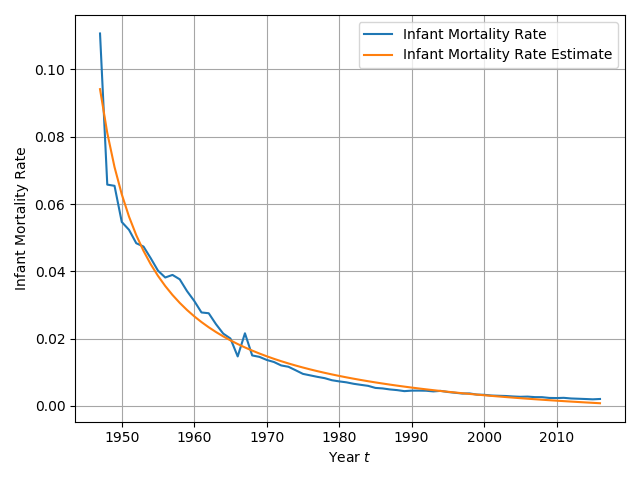
\includegraphics[width=0.50\textwidth]{\FigureDir/mortality/smooth_0/_infant_mortality_rate_predicted.png}
         \end{tabular}
      \end{threeparttable}
   }
\end{figure}

\par I begin the non-infant mortality rate estimation by fitting the yearly distributions using a generalized beta 2 distribution. The pdf for this distribution is defined in \ref{eq:gb2_pdf}. This is the same distribution used to fit fertility estimates. I choose to use a generalized beta 2 distribution rather than an exponential, which is what the data appears to follow, because the fit is almost identical but there is no discernable trend in parameter estimates for an exponential distribution but there is a very clear trend for the generalized beta 2 distribution.

\par As with fertility rates, because the generalized beta 2 is a pdf but mortality rates are not a pdf, I also have to add in a scale parameter. I estimate mortality parameters from 1970 to 2014, the same years as for fertility rates.

\par The fit of the model in selected years can be seen in \autoref{fig:\thesubsubsection.2}. The estimated distribution has a very close fit to the true data. This is true for all years, unlike the fertility estimates which do not fit the tails properly for recent data.

\par Parameter estimates and their fit over time can be seen in \autoref{fig:\thesubsubsection.3}. In order to ensure estimated trends converge over time, I fit these parameter estimates to logistic functions. The logistic function can be seen in \ref{eq:logistic_fn}. This is the same distribution used to fit fertility parameters.

\begin{figure}[!ht]
   \centering
   \caption{\label{fig:\thesubsubsection.2}Mortality Estimated by Generalized Beta 2}
   \begin{subfigure}{0.5\textwidth}
      \centering
      \includegraphics[width=\textwidth]{\FigureDir/mortality/smooth_0/1970.png}
      \caption{1970}
   \end{subfigure}% <-- this "%" symbol is important
   ~ % <-- this "~" symbol is important
   \begin{subfigure}{0.5\textwidth}
      \centering
      \includegraphics[width=\textwidth]{\FigureDir/mortality/smooth_0/1990.png}
      \caption{1990}
   \end{subfigure}%
   \newline
   \begin{subfigure}{0.5\textwidth}
      \centering
      \includegraphics[width=\textwidth]{\FigureDir/mortality/smooth_0/2000.png}
      \caption{2000}
   \end{subfigure}%
   ~ % <-- this "~" symbol is important
   \begin{subfigure}{0.5\textwidth}
      \centering
      \includegraphics[width=\textwidth]{\FigureDir/mortality/smooth_0/2014.png}
      \caption{2014}
   \end{subfigure}%
\end{figure}

\begin{figure}[!ht]
	\centering
   \caption{\label{fig:\thesubsubsection.3}Mortality Generalized Beta 2 Parameter Estimates}
		\begin{subfigure}{0.5\textwidth}
			\centering
			\includegraphics[width=\textwidth]{\FigureDir/mortality/smooth_0/_a_predicted.png}
			\caption{\(a\)}
		\end{subfigure}% <-- this "%" symbol is important
		~ % <-- this "~" symbol is important
		\begin{subfigure}{0.5\textwidth}
			\centering
			\includegraphics[width=\textwidth]{\FigureDir/mortality/smooth_0/_b_predicted.png}
			\caption{\(b\)}
		\end{subfigure}%
		\newline
		\begin{subfigure}{0.5\textwidth}
			\centering
			\includegraphics[width=\textwidth]{\FigureDir/mortality/smooth_0/_p_predicted.png}
			\caption{\(p\)}
		\end{subfigure}%
		~ % <-- this "~" symbol is important
		\begin{subfigure}{0.5\textwidth}
			\centering
			\includegraphics[width=\textwidth]{\FigureDir/mortality/smooth_0/_q_predicted.png}
			\caption{\(q\)}
      \end{subfigure}%
      \newline
		\begin{subfigure}{0.5\textwidth}
			\centering
			\includegraphics[width=\textwidth]{\FigureDir/mortality/smooth_0/_scale_predicted.png}
			\caption{Scale}
		\end{subfigure}%
\end{figure}

\par With the parameters from the logistic function estimated, we can now test the quality of our model fit. Comparisons of the models estimated with true data can be seen in \autoref{fig:\thesubsubsection.4}. The first panel shows the trend in true mortality rates from 1970-2014; the second panel shows the trend in model mortality rates from 1970-2014 using the logistic estimates of the generalized beta 2 parameters; the third panel shows the first two trends overlaid, with true data in red and model data in blue; and the fourth panel shows select estimates from the model.

\par From the first three panels, we can see that the model represents the general trends in mortality rates properly. 

\par The fourth panel gives us an indication of how mortality will evolve over time. We can see consistent decline in mortality from 1990 to 2000 to 2014, which follows the same trend as the true data. With our model we now also have the ability to forecast future mortality rates. Our model forecasts that by 2050 mortality rates will continue their trend downward. We also see that the logistic functional form leads to a convergence in mortality rates by 2050 - the estimate for 2100 is almost exactly overlaid with the estimate for 2050.

\begin{figure}[!ht]
   \centering
   \caption{\label{fig:\thesubsubsection.4}Mortality Generalized Beta 2 Model Fit}
   \begin{subfigure}{0.5\textwidth}
      \centering
      \includegraphics[width=\textwidth]{\FigureDir/mortality/smooth_0/_aggregate_true.png}
      \caption{Data, 1970 (light) - 2014 (dark)}
   \end{subfigure}% <-- this "%" symbol is important
   ~ % <-- this "~" symbol is important
   \begin{subfigure}{0.5\textwidth}
      \centering
      \includegraphics[width=\textwidth]{\FigureDir/mortality/smooth_0/_aggregate_predicted.png}
      \caption{Model}
   \end{subfigure}%
   \newline
   \begin{subfigure}{0.5\textwidth}
      \centering
      \includegraphics[width=\textwidth]{\FigureDir/mortality/smooth_0/_aggregate_overlay_predicted.png}
      \caption{Model (Blue) Overlays Data (Red)}
   \end{subfigure}%
   ~ % <-- this "~" symbol is important
   \begin{subfigure}{0.5\textwidth}
      \centering
      \includegraphics[width=\textwidth]{\FigureDir/mortality/smooth_0/_2100.png}
      \caption{Model Forecasts}
   \end{subfigure}%
\end{figure}

% %%%%%%%%%%%%%%%%%%%%%%%%%%%%%%%%%%%%%%%%%%%%%%%%%
% \subsubsection{Forecasting Demographics - Immigration Rates}
% %%%%%%%%%%%%%%%%%%%%%%%%%%%%%%%%%%%%%%%%%%%%%%%%%

\subsubsection{Immigration Rates}

\par Estimating the evolution of immigration rates over time poses more of a challenge than fertility or mortality rates. While fertility and mortality rates can be estimated using a generalized beta 2 distribution, immigration rates following a distribution that is difficult to model without a mixture method. To get around this, I instead model the evolution in immigration rates for each age. While this no longer allows for the use of a simple distribution and clear parameter evolutions over time for the entire set of data, it seems like a more reasonable way to fit the data than to fit a mixture model with a large number of distributions.

\par To fit the evolution of immigration rates for each age, I estimate the trend from 1997-2014 using linear regression, then forecast using an exponential distribution that matches the slope of the linear regression in 2014 and is assumed to plateau in 15 years at a value 10\% beyond the last value in the data. The exponential I fit is defined as

\begin{equation}
   f(x|a, b, c, d, p, s, \beta_0, \beta_1) = e^{a(x-s)^2 + b(x-s) + c} + p
\end{equation}

\begin{align*}
   s.t. \hspace{5mm} &\left.\pdv{f}{x}\right|_{x=s} = \beta_1 \tag{cond. 1} \label{c1} \\
   &f(s) = \beta_0 + \beta_1 s \tag{cond. 2} \label{c2} \\
   &\left.\pdv{f}{x}\right|_{x=s + 15} \approx 0 \tag{cond. 3} \label{c3} \\
   &f(s + 15) = d \cdot f(s) \tag{cond. 4} \label{c4}
\end{align*}

\par where \(a, b\), and \(c\) are parameters to estimate, \(p\) shifts the curve so we can estimate \(c\) (this is explained in the derivation), \(s\) gives the last year of data, \(\beta_0\) and \(\beta_1\) are the OLS estimates from fitting the data, and we define \(d\) such that

\[
   d = \left\{\begin{matrix}
      0.9 & \text{if} & (\beta < 0 \text{ and } f(s) > 0) \text{ or } (\beta > 0 \text{ and } f(s) < 0) \\
      1.1 & \text{if} & (\beta < 0 \text{ and } f(s) < 0) \text{ or } (\beta > 0 \text{ and } f(s) > 0) \\
      1 & \text{if} & \beta = 0
   \end{matrix}\right.
\]

\par For notational simplicity, I will define \(\beta = \beta_0 + \beta_1s\). We therefore have from \ref{c2} that \(e^c + p = \beta \Leftrightarrow c = \log(\beta - p)\). In order to ensure that we can compute \(c\), we set \(p < \beta\).

\par Using \(\pdv{f}{x} = (2a(x-s) + b)e^{a(x-s)^2 + b(x-s) + c}\) and \ref{c1}, we have \(be^c = \beta_1 \Leftrightarrow b = \frac{\beta_1}{\beta - p}\).

\par From \ref{c3} we have \((2a(15) + b)(f(x+15) - p) \approx 0\). Because the derivative cannot actually become 0, we can choose a value very close to 0 to estimate this curve numerically. We will label this value \(\epsilon\). Plugging in the value for \(f(x+15)\) from \ref{c4}, and recalling that \(f(s) = \beta_0 + \beta_1s = \beta\), we have \(\left(2a(15) + \frac{\beta_1}{\beta - p}\right)(d\cdot \beta - g) = \epsilon \Leftrightarrow a = \frac{1}{30}\left(\frac{\epsilon}{d\cdot\beta-g} - \frac{\beta_1}{\beta - p}\right)\). At 2030, we assume that the estimate stays constant for future years.

\par We therefore have the following:
\[
   \left\{
      p < \beta,
      a = \frac{1}{30}\left(\frac{\epsilon}{d\cdot\beta - g} - \frac{\beta_1}{\beta - p}\right),
      b = \frac{\beta_1}{\beta - p},
      c = \log(\beta - p)
   \right\}
\]

\par where \(\beta = \beta_0 + \beta_1s\).

\par The fit of the model for selected ages can be seen in \autoref{fig:\thesubsubsection.1}. Unlike fertility and mortality rates, fertility rates by age appear not to have as predictable a trend. However, the linear regression model with exponential forecasts seems sufficient to have reasonable forecasts for the short term.

\begin{figure}[!ht]
   \centering
   \caption{\label{fig:\thesubsubsection.1}Immigration Estimated by Linear Regression and Forecasted by Exponential}
   \begin{subfigure}{0.5\textwidth}
      \centering
      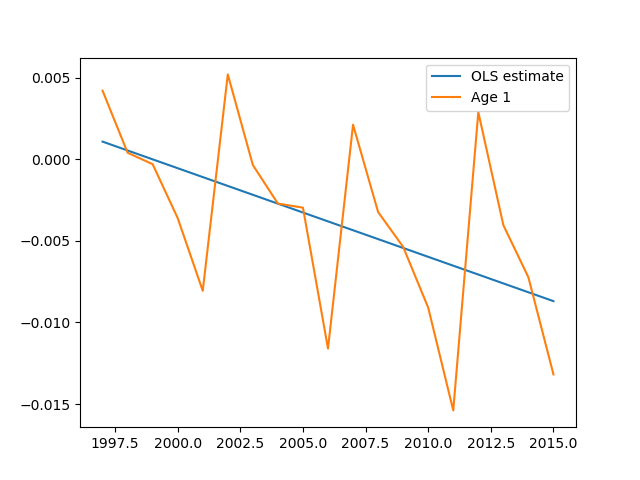
\includegraphics[width=\textwidth]{\FigureDir/immigration/age_forecasts/1.png}
      \caption{Age 1}
   \end{subfigure}% <-- this "%" symbol is important
   ~ % <-- this "~" symbol is important
   \begin{subfigure}{0.5\textwidth}
      \centering
      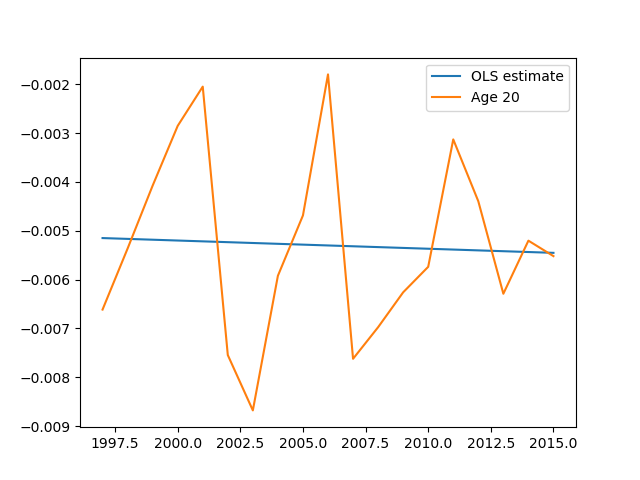
\includegraphics[width=\textwidth]{\FigureDir/immigration/age_forecasts/20.png}
      \caption{Age 20}
   \end{subfigure}%
   \newline
   \begin{subfigure}{0.5\textwidth}
      \centering
      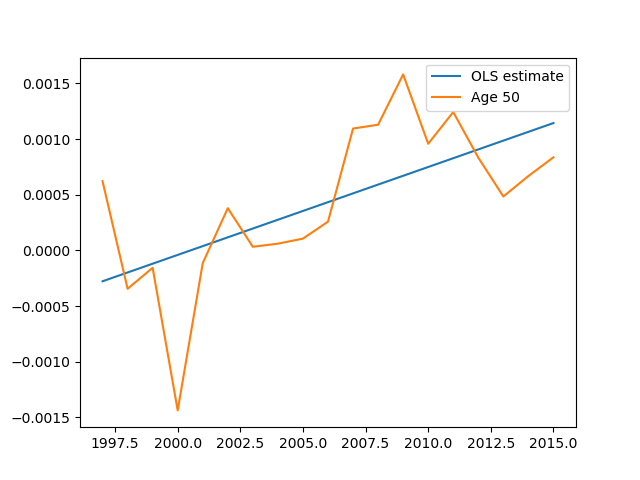
\includegraphics[width=\textwidth]{\FigureDir/immigration/age_forecasts/50.png}
      \caption{Age 50}
   \end{subfigure}%
   ~ % <-- this "~" symbol is important
   \begin{subfigure}{0.5\textwidth}
      \centering
      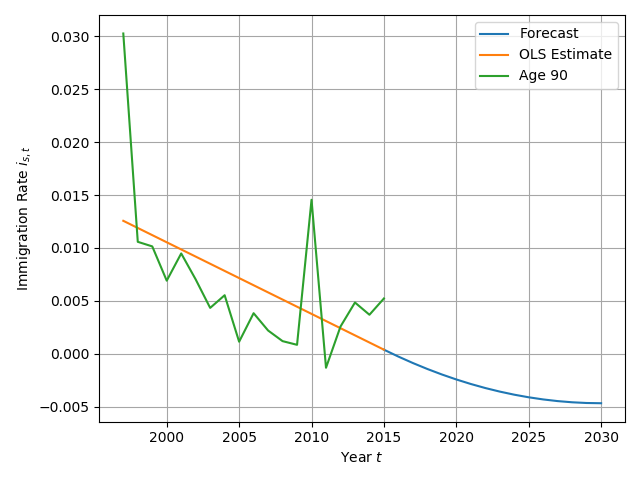
\includegraphics[width=\textwidth]{\FigureDir/immigration/age_forecasts/90.png}
      \caption{Age 90}
   \end{subfigure}%
\end{figure}

\par With the parameters from the linear regression and exponential estimated, we can now test the quality of our model fit. Comparisons of the models estimated with true data can be seen in \autoref{fig:\thesubsubsection.2}. The first panel shows the trend in true immigration rates from 1997-2014; the second panel shows the trend in model immigration rates from 1997-2014; the third panel shows the first two trends overlaid, with true data in red and model data in blue; and the fourth panel shows select estimates from the model.

\par From the first three panels, we can see that the model represents the general trends in immigration rates properly, although with reduced variance. 

\par The fourth panel gives us an indication of how immigration will evolve over time. We can see consistent decline in immigration from 1990 to 2000 to 2014 for the young and the old, with little change in immigration rates for other ages, which follows the same trend as the true data. With our model we now also have the ability to forecast future immigration rates. Our model forecasts that by 2050 immigration rates will continue their trend downward for the old. In order to prevent population estimates from declining too rapidly I choose to increase immigration rates for the 0 year old population rather than let it continue to decline. Other ages seem to have relatively unchanged immigration rates over time. We can also see that following our construction, we have a convergence in immigration rates by 2030.

\begin{figure}[!ht]
   \centering
   \caption{\label{fig:\thesubsubsection.2}Immigration Estimated by Linear Regression and Forecasted by Exponential}
   \begin{subfigure}{0.5\textwidth}
      \centering
      \includegraphics[width=\textwidth]{\FigureDir/immigration/smooth_0/_aggregate_true.png}
      \caption{Data, 1970 (light) - 2014 (dark)}
   \end{subfigure}% <-- this "%" symbol is important
   ~ % <-- this "~" symbol is important
   \begin{subfigure}{0.5\textwidth}
      \centering
      \includegraphics[width=\textwidth]{\FigureDir/immigration/smooth_0/_aggregate_predicted.png}
      \caption{Model}
   \end{subfigure}%
   \newline
   \begin{subfigure}{0.5\textwidth}
      \centering
      \includegraphics[width=\textwidth]{\FigureDir/immigration/smooth_0/_aggregate_overlay_predicted.png}
      \caption{Model (Blue) Overlays Data (Red)}
   \end{subfigure}%
   ~ % <-- this "~" symbol is important
   \begin{subfigure}{0.5\textwidth}
      \centering
      \includegraphics[width=\textwidth]{\FigureDir/immigration/smooth_0/_2100.png}
      \caption{Model Forecasts}
   \end{subfigure}%
\end{figure}

% %%%%%%%%%%%%%%%%%%%%%%%%%%%%%%%%%%%%%%%%%%%%%%%%%
% \subsubsection{Forecasting Demographics - Population}
% %%%%%%%%%%%%%%%%%%%%%%%%%%%%%%%%%%%%%%%%%%%%%%%%%

\subsubsection{Population}

\par Using our fertility, mortality, and immigration estimates, we can now use the population evolution described in \ref{eq:pop_evolution} to forecast future population given an initial year of population data.

\par We will first analyze quality of fit on past data. I test by beginning with 1970 population data and comparing the true population evolution against the population evolution forecasted by the model. Selected years of the transition from 1970 to 2017, the most recent population data, can be seen in \autoref{fig:\thesubsubsection.1}. We can see in the first year of the model that there is a slight overestimate of births. This persists over time for this particular cohort, as the mortality rate should not be compensating for this. However, this slight overestimate is actually a rise in population that is is seen to occur just a few years later in the true data, when looking at the figure from 1985. The model does an accurate job of representing the inflection point in population that occurs around 1974 in the real data, and 1972 in the forecast. Looking at the figure from 2000, we can see that the model also accurately fits the inflection point in population around 1997. However, we begin to see that there a few ages where the model is overestimating the population and other ages where it is underestimating the population. The final figure is for 2017. This is 47 years after the start. The model appears to fit the data well and reflects the inflection points in the data. 

\begin{figure}[!ht]
   \centering
   \caption{\label{fig:\thesubsubsection.1}Forecasted Versus True Population Initial Population Set to 1970}
   \begin{subfigure}{0.5\textwidth}
      \centering
      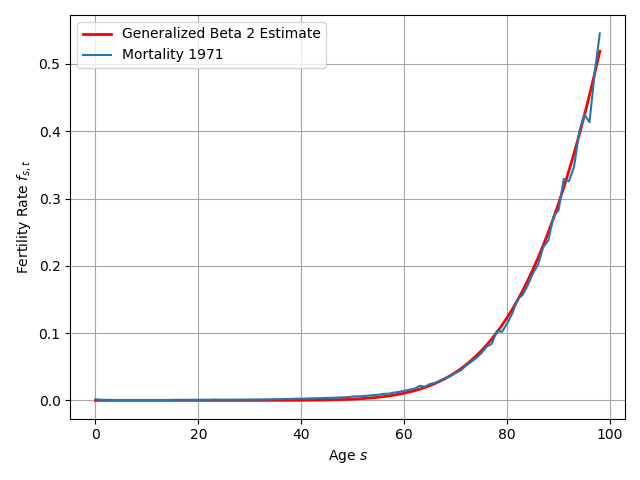
\includegraphics[width=\textwidth]{\FigureDir/population_forecasts/start_1970/1971.png}
      \caption{1971}
   \end{subfigure}% <-- this "%" symbol is important
   ~ % <-- this "~" symbol is important
   \begin{subfigure}{0.5\textwidth}
      \centering
      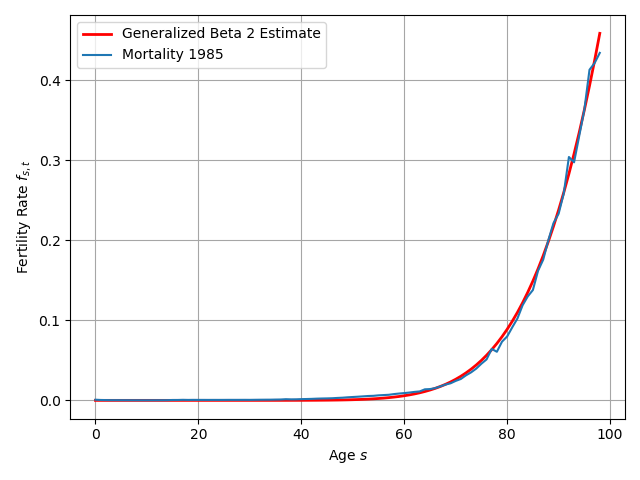
\includegraphics[width=\textwidth]{\FigureDir/population_forecasts/start_1970/1985.png}
      \caption{1985}
   \end{subfigure}%
   \newline
   \begin{subfigure}{0.5\textwidth}
      \centering
      \includegraphics[width=\textwidth]{\FigureDir/population_forecasts/start_1970/2000.png}
      \caption{2000}
   \end{subfigure}%
   ~ % <-- this "~" symbol is important
   \begin{subfigure}{0.5\textwidth}
      \centering
      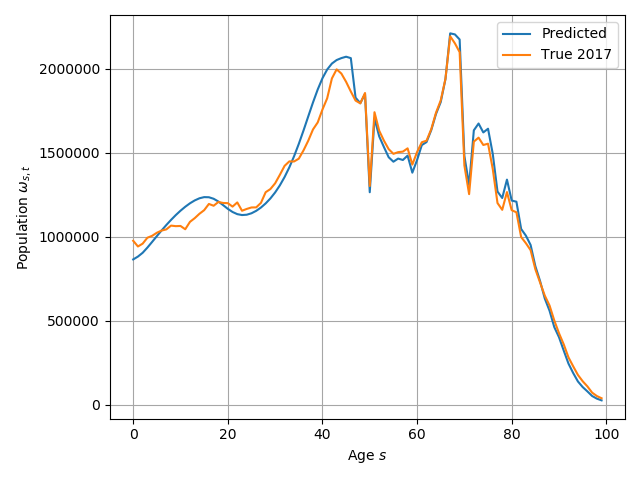
\includegraphics[width=\textwidth]{\FigureDir/population_forecasts/start_1970/2017.png}
      \caption{2017}
   \end{subfigure}%
\end{figure}

% %%%%%%%%%%%%%%%%%%%%%%%%%%%%%%%%%%%%%%%%%%%%%%%%%
% \subsubsection{Forecasting Demographics - Alternate}
% %%%%%%%%%%%%%%%%%%%%%%%%%%%%%%%%%%%%%%%%%%%%%%%%%

\subsubsection{Alternate Forecasting}

\par The final model we consider is a principal components analysis (PCA) forecasting model. The model uses a functional variation on the non-parametric PCA method to solve an orthonormal basis that maximizes the explained variance in the historical fertility, mortality, and immigration data. It then uses a univariate robust ARIMA model to forecast these values over time. Forecasts are made using the \(R\) package Demographics (\cite{alt_demo}) which is described in detail in \cite{alt_demo_paper}. \autoref{fig:alt_demog} includes fertility forecasts in the first panel, mortality forecasts in the second panel, and immigration forecasts in the third panel using the PCA approach.

\begin{figure}[!ht]
   \caption{\label{fig:alt_demog}Demographics Forecasted by PCA}
   \begin{subfigure}{0.5\textwidth}
      \centering
      \includegraphics[width=\textwidth]{\FigureDir/fertility/alternate/_2100.png}
      \caption{Fertility Rates}
   \end{subfigure}% <-- this "%" symbol is important
   ~ % <-- this "~" symbol is important
   \begin{subfigure}{0.5\textwidth}
      \centering
      \includegraphics[width=\textwidth]{\FigureDir/mortality/alternate/_2100.png}
      \caption{Mortality Rates}
   \end{subfigure}
   \newline
   \begin{subfigure}{0.5\textwidth}
      \centering
      \includegraphics[width=\textwidth]{\FigureDir/immigration/alternate/_2100.png}
      \caption{Immigration Rates}
   \end{subfigure}
\end{figure}

% %%%%%%%%%%%%%%%%%%%%%%%%%%%%%%%%%%%%%%%%%%%%%%%%%
% \subsubsection{Forecasting Demographics - Population Forecasts}
% %%%%%%%%%%%%%%%%%%%%%%%%%%%%%%%%%%%%%%%%%%%%%%%%%

\subsubsection{Population Forecasts}

\par We now move to forecasting future populations. We can see how population will evolve over time in \autoref{fig:\thesubsubsection.2}. We can see that the population growth rate becomes negative by the steady state. This causes population to converge to 0 by 2500. This is true for all three models we consider with evolving population when simulating in the overlapping generations model. This result should caution any user of this model - it seems unlikely that fertility rates would not endogenously increase in response to persistently declining populations. We also may expect an endogenous immigration response.

\par We can see the distribution of the population at select years in the future for each model in \autoref{fig:\thesubsubsection.3}. We can see that for the partial-dynamic and full-dynamic model, the modal age of the population increases over time until it peaks at around 75 years old. This result indicates Japan faces a massive hurdle with its aging population.

\par These results differ noticeably from the forecasts from the non-parametric PCA model. Because fertility rates see rapid growth through 2100, population explodes. This causes the population distribution to weight heavily towards younger ages. Decreasing mortality rates also help the population grow over time. This leads to a positive population growth rate in the long-run. While these results are surprising, we choose to limit demographic forecasts to 2050 for the PCA model in the overlapping generations simulations in order to maintain consistency between demographic models. It is also clear that forecasts 30 years or further into the future will have such high uncertainty that assuming convergence at this point will be no less accurate than assuming a continuation in trends. Demographic forecasts when assuming convergence in 2050 can be seen in \autoref{fig:steady_state_demographics} and lead to a negative population growth rate in the steady state. The model leads to a modal age of around 90 in the steady state.

\begin{figure}[!ht]
   \centering
   \caption{\label{fig:\thesubsubsection.2}Forecasted Population}
   \scalebox{1}{
      \begin{threeparttable}
         \begin{tabular}{c}
            \includegraphics[width=0.50\textwidth]{\FigureDir/population_forecasts/start_2017/predicted_basic.png}
         \end{tabular}
      \end{threeparttable}
   }
\end{figure}

\begin{figure}[!ht]
   \centering
   \caption{\label{fig:\thesubsubsection.3}Forecasted Population and Population Distribution}
   \scalebox{1}{
      \begin{threeparttable}
         \begin{tabular}{cc}
            \includegraphics[width=0.50\textwidth]{\FigureDir/population_forecasts/start_2017/predicted_proportion_basic.png} & \includegraphics[width=0.50\textwidth]{\FigureDir/population_forecasts/start_2017/predicted_proportion_parametric.png}
         \end{tabular}
      \end{threeparttable}
   }
   \scalebox{1}{
      \begin{threeparttable}
         \begin{tabular}{c}
            \includegraphics[width=0.50\textwidth]{\FigureDir/population_forecasts/start_2017/predicted_proportion_alt.png}
         \end{tabular}
      \end{threeparttable}
   }
\end{figure}

% %%%%%%%%%%%%%%%%%%%%%%%%%%%%%%%%%%%%%%%%%%%%%%%%%
% \subsubsection{Forecasting Demographics - Steady State}
% %%%%%%%%%%%%%%%%%%%%%%%%%%%%%%%%%%%%%%%%%%%%%%%%%

\subsubsection{Steady State}

\par We can see steady state demographic results for the four models in \autoref{fig:steady_state_demographics}. Following the methods of \cite{DE2018}, we artificially impose that the population reaches its steady state distribution at \(t=120\). We do this by adjusting immigration rates such that \ref{eq:pop_evolution} stabilizes. The first column of the results gives the true steady state population (the derivation of this is described in detail in \cite{DE2018}) and the population at \(t=120\), when we force convergence. As described previously, we can see how dramatically the population distribution varies between the four models. In particular, we can see the population distribution from the PCA model when we force convergence of fertility, mortality, and immigration rates in 2050. We see that the population distribution becomes very highly skewed, with almost all the population being those over 60. The modal age in this model is almost 90 years old. The distributions for the static, partial-dynamic, and full-dynamic models are the same as described above. The third column gives the transitions of the demographic distributions over time.

\par In the second column, we can see steady state and adjusted immigration rates. In particular, it is noteworthy how negative the immigration rates are for babies and the elderly. For babies, this result may be coming from the emigration of young adults. These young adults are having a large portion of the babies being born, which could explain why it appears that even if only a small portion of young adults are leaving, if they make up a large portion of new parents, that would cause the immigration rate for babies to become extremely negative. This could also be an issue arising from the fertility data. The results for the elderly population are not surprising. Given the small proportion of the population that is subject to these unusual results, it is plausible that small disparities between the fertility, mortality, and population data could lead to apparently large immigration rates for the elderly population.

\par Comparing the steady state immigration results, there do not appear to be noteworthy differences between the results of the static, partial-dynamic, and full-dynamic models. The largest difference appears to be that the full-dynamic model has slightly lower immigration rates for the elderly population. The largest difference appears in the PCA model. We see that immigration rates are very near to zero for all ages except babies. However, immigration rates for babies become very negative: almost 80\% of all babies appear to be leaving the country in the model. This largely explain why the demographic distribution ends up with such a high proportion of older individuals, as almost all babies end up leaving the country.

\begin{figure}[!ht]
   \centering
   \caption{\label{fig:steady_state_demographics}Population Steady State, and Adjustments, and Transition Path}
   \textbf{Static Demographics}
   \begin{subfigure}{0.33\textwidth}
      \centering
      \includegraphics[width=\textwidth]{\DemoDir/static/OrigVsFixSSpop.png}
   \end{subfigure}% <-- this "%" symbol is important
   ~ % <-- this "~" symbol is important
   \begin{subfigure}{0.33\textwidth}
      \centering
      \includegraphics[width=\textwidth]{\DemoDir/static/OrigVsAdjImm.png}
   \end{subfigure}% <-- this "%" symbol is important
   ~ % <-- this "~" symbol is important
   \begin{subfigure}{0.33\textwidth}
      \centering
      \includegraphics[width=\textwidth]{\DemoDir/static/PopDistPath.png}
   \end{subfigure}

   \textbf{Partial-Dynamic Demographics}
   \begin{subfigure}{0.33\textwidth}
      \centering
      \includegraphics[width=\textwidth]{\DemoDir/dynamic_partial/OrigVsFixSSpop.png}
   \end{subfigure}% <-- this "%" symbol is important
   ~ % <-- this "~" symbol is important
   \begin{subfigure}{0.33\textwidth}
      \centering
      \includegraphics[width=\textwidth]{\DemoDir/dynamic_partial/OrigVsAdjImm.png}
   \end{subfigure}% <-- this "%" symbol is important
   ~ % <-- this "~" symbol is important
   \begin{subfigure}{0.33\textwidth}
      \centering
      \includegraphics[width=\textwidth]{\DemoDir/dynamic_partial/PopDistPath.png}
   \end{subfigure}

   \textbf{Full-Dynamic Demographics}
   \begin{subfigure}{0.33\textwidth}
      \centering
      \includegraphics[width=\textwidth]{\DemoDir/dynamic_full/OrigVsFixSSpop.png}
   \end{subfigure}% <-- this "%" symbol is important
   ~ % <-- this "~" symbol is important
   \begin{subfigure}{0.33\textwidth}
      \centering
      \includegraphics[width=\textwidth]{\DemoDir/dynamic_full/OrigVsAdjImm.png}
   \end{subfigure}% <-- this "%" symbol is important
   ~ % <-- this "~" symbol is important
   \begin{subfigure}{0.33\textwidth}
      \centering
      \includegraphics[width=\textwidth]{\DemoDir/dynamic_full/PopDistPath.png}
   \end{subfigure}

   \textbf{Alternate Full-Dynamic Demographics}
   \begin{subfigure}{0.33\textwidth}
      \centering
      \includegraphics[width=\textwidth]{\DemoDir/dynamic_full_alternate/OrigVsFixSSpop.png}
      \caption{\\ \shortstack{Original vs. Adjusted\\SS Population Distribution}}
   \end{subfigure}% <-- this "%" symbol is important
   ~ % <-- this "~" symbol is important
   \begin{subfigure}{0.33\textwidth}
      \centering
      \includegraphics[width=\textwidth]{\DemoDir/dynamic_full_alternate/OrigVsAdjImm.png}
      \caption{\\ \shortstack{Original vs. Adjusted\\Immigration Rates}}
   \end{subfigure}% <-- this "%" symbol is important
   ~ % <-- this "~" symbol is important
   \begin{subfigure}{0.33\textwidth}
      \centering
      \includegraphics[width=\textwidth]{\DemoDir/dynamic_full_alternate/PopDistPath.png}
      \caption{\\ \shortstack{Population Distribution\\Along Time Path}}
   \end{subfigure}
\end{figure}

% %%%%%%%%%%%%%%%%%%%%%%%%%%%%%%%%%%%%%%%%%%%%%%%%%
% \section{Results}
% %%%%%%%%%%%%%%%%%%%%%%%%%%%%%%%%%%%%%%%%%%%%%%%%%

\newpage
\section{Results}

% %%%%%%%%%%%%%%%%%%%%%%%%%%%%%%%%%%%%%%%%%%%%%%%%%
% \subsection{Results - Demographics}
% %%%%%%%%%%%%%%%%%%%%%%%%%%%%%%%%%%%%%%%%%%%%%%%%%

\subsection{Demographics}

\par We consider the demographic transitions of the four models. Steady state population distributions can be seen in \autoref{fig:steady_state_demographics}. As we move from the first to the last model, the steady state population distribution becomes increasingly negatively skewed. The transition from the static to the partial-dynamic model reflects the low fertility rate of the current population, which is below replacement level (we know this because the steady-state partial-dynamic population has a negative growth rate). The transition from the partial-dynamic to both full-dynamic models reflects the downward trend in fertility (\autoref{fig:3.1.1.3}), mortality (\autoref{fig:3.1.2.4}), and immigration (\autoref{fig:3.1.3.2}) rates over time. As these rates decrease, the population will decrease and the proportion of the population that is younger (older) will decrease (increase).

\par While these distinctions are interpretable, the reason for the distinction between the demographic outcomes of the two full-dynamic models is not as clear. While the third model is constructed to fit the shape of demographic curves very closely, the PCA model is non-parametric. This allows the model to extract more information from the data, but it also allows it to behave in unpredictable, possibly incorrect ways. This can be seen in \autoref{fig:alt_demog}. The third model forces the fertility rates to follow a single-modal model. However, the fourth model ends up predicting that fertility will become bi-modal in the future. This prediction is hard to justify given that the predictions are not endogenous and thus cannot include a change in preferences. Further, the model predicts that fertility rates will continue to increase for older ages. While looking at data for any particular older age appears to indicate fertility rates will continue increasing (although perhaps not quite as much as this model predicts), when considering the trend of the entire distribution of fertility rates, as the parametric model does, this seems somewhat unlikely.

\par One overarching explanation may be that PCA does not assume that the models will converge over time. This is what allows the fertility rates to continue increasing, the mortality rates to all converge to zero over time, and the immigration rates to decline to very low values.\footnote{It should be noted that the PCA itself does not put bounds on any rates. Fertility rates are bounded below at zero, mortality rates are bounded between zero and one, and immigration rates are bounded between minus one and one after running the PCA.} The parametric model seems to be preferable in this case, as historical data seems to show a trend towards convergence. However, the PCA analysis does consider the entire dataset so perhaps there is more value to this analysis than appears at first glance.

\par We now move to the results from the overlapping generations model. It should be noted that the static model seems to be giving results that are an order of magnitude too small as of the writing of this paper. This may be caused by choosing not to alter immigration rates to stabilize population levels in the steady state, making the model internally inconsistent. Regardless, this does not alter qualitative comparisons of the results of the three dynamic models.

% %%%%%%%%%%%%%%%%%%%%%%%%%%%%%%%%%%%%%%%%%%%%%%%%%
% \section{Results - Steady-State}
% %%%%%%%%%%%%%%%%%%%%%%%%%%%%%%%%%%%%%%%%%%%%%%%%%
\subsection{Steady-State}

\par Steady-state results giving percent deviations from the static demographic model can be seen below. Steady-state results for each model can be seen in \aref{sec:A.2.2}. We focus on the percent deviation results, treating the static model as a baseline.

\par \autoref{fig:ss_consumption_pct} and \autoref{fig:ss_savings_pct} show results for steady-state consumption and savings, respectively. The left panel gives results from the static (baseline) model. The right panel gives percent deviations from the baseline for the other three models considered. We can see that all four models follow a similar trend of an increase in consumption and savings until around age 70, when consumption and savings peak and then subsequently decline. However, what is noteworthy is the distinction between the static and dynamic models. The dynamic models are everywhere higher in both consumption and savings relative to the static model. There is also an even higher peak in these models at older ages. The results are especially apparent for the PCA model. While it is also everywhere higher than the static model, it is lower than the partial- and full-dynamic models at all ages until around 80 for consumption and 70 for savings. It then quickly surpasses the other two models and peaks at much higher levels of consumption and savings around age 90. This is likely explained by the very low mortality rates predicted by the PCA model (these predictions can be seen in \autoref{fig:alt_demog}).

\begin{figure}[H]
   \caption{\label{fig:ss_consumption_pct}Steady-State Consumption}
   \begin{subfigure}{0.5\textwidth}
      \centering
      \includegraphics[width=\textwidth]{\SSDir/pct_change/images/SS_c_static.png}
      \caption{Static Demographics}
   \end{subfigure}%
   ~
   \begin{subfigure}{0.5\textwidth}
      \centering
      \includegraphics[width=\textwidth]{\SSDir/pct_change/images/SS_c.png}
      \caption{All Other Demographics (\% Deviation from Static)}
   \end{subfigure}
\end{figure}

\begin{figure}[H]
   \caption{\label{fig:ss_savings_pct}Steady-State Savings}
   \begin{subfigure}{0.5\textwidth}
      \centering
      \includegraphics[width=\textwidth]{\SSDir/pct_change/images/SS_b_static.png}
      \caption{Static Demographics}
   \end{subfigure}%
   ~
   \begin{subfigure}{0.5\textwidth}
      \centering
      \includegraphics[width=\textwidth]{\SSDir/pct_change/images/SS_b.png}
      \caption{All Other Demographics (\% Deviation from Static)}
   \end{subfigure}
\end{figure}

\par \autoref{fig:ss_labor_pct} shows results for steady-state labor supply. Steady-state labor appears almost inverted relative to steady-state consumption and savings. There is a decline in labor supply over time until it troughs at around age 70, at which point it subsequently increases. Again, it is important to distinguish between the static and dynamic models. The dynamic models are everywhere lower in labor supply relative to the static model. The dynamic models have even more extreme declines in labor at older ages. These results are more apparent for the PCA model, where the reduction in labor is less than the reduction in the partial- and full-dynamic models until around age 80, when it drops to be significantly below the declines of the other models.

\begin{figure}[H]
   \caption{\label{fig:ss_labor_pct}Steady-State Labor}
   \begin{subfigure}{0.5\textwidth}
      \centering
      \includegraphics[width=\textwidth]{\SSDir/static/images/SS_n.png}
      \caption{Static Demographics}
   \end{subfigure}%
   ~
   \begin{subfigure}{0.5\textwidth}
      \centering
      \includegraphics[width=\textwidth]{\SSDir/pct_change/images/SS_n.png}
      \caption{All Other Demographics (\% Deviation from Static)}
   \end{subfigure}
\end{figure}

%\par \autoref{fig:ss_consumption} shows results for steady-state consumption and savings. We can see that the trend is almost identical in all four demographic models. However, the levels differ by model. The static model gives consumption and savings at about one-tenth the rate of the other models. This likely reflects the higher population of this model. The first model has constant population over time, meaning bequests will be the same proportion of the former population's income as the current population. However, the second through fourth models have negative population growth in the steady state. This will lead bequests to be a larger portion of the future population's income. This will allow them to consume and save more over their lifetimes.

%\par \autoref{fig:ss_labor} shows results for steady-state labor supply. The differences between the models again likely reflects their differing population growth rates. Because agents in the first model have less endowments from bequests relative to income, they are forced to work more for a similar level of consumption and savings. In the second through fourth models, the higher level of endowments from bequests relative to income means agents have to work less for a similar level of consumption and savings.

% %%%%%%%%%%%%%%%%%%%%%%%%%%%%%%%%%%%%%%%%%%%%%%%%%
% \section{Results - Time Path}
% %%%%%%%%%%%%%%%%%%%%%%%%%%%%%%%%%%%%%%%%%%%%%%%%%

\subsection{Time Path}
\par Time path results giving percent deviations from the static demographic model can be seen below. Time path results for each model can be seen in \aref{sec:A.2.3}. We focus on the percent deviation results, treating the static model as a baseline.

\par We start our discussion by considering aggregate output, aggregate capital, and aggregate consumption. Aggregate output results can be seen in \autoref{fig:tp_Y_pct}. Aggregate capital results can be seen in \autoref{fig:tp_K_pct}. Aggregate consumption results can be seen in \autoref{fig:tp_C_pct}. These three aggregates all follow very similar time paths. In the baseline model, they all begin at relatively low levels, increase rapidly and then quickly stabilize to their steady state levels in around 30 years. The three models with evolving population have remarkably different time paths relative to the static model in the short-term. They all begin with significantly higher levels of all three aggregates, but then similarly converge to steady state levels within around 30 years and these levels are very close to the static model. Results are all within a few percentage points by this convergence.

\par While the three models converge to similar levels in the long-run, the transition itself is particularly relevant. All three dynamic models are everywhere higher in output, capital, and consumption over the short- and medium-run than in the static model. Further, both the partial- and full-dynamic models have few deviations in these variables in the long-run. The PCA model, however, appears to have small but persistent deviations from its long-run trend, particularly for output. We show only the first 50 years of the transition for output to emphasize the short- and medium-run behavior of the model, as well as the deviations in the PCA model.

\begin{figure}[H]
   \caption{\label{fig:tp_Y_pct}Time Path of Aggregate Output \(\hat{Y}_t\)}
   \begin{subfigure}{0.5\textwidth}
      \centering
      \includegraphics[width=\textwidth]{\TPDir/static/images/TP_Y_path.png}
      \caption{Static Demographics}
   \end{subfigure}%
   ~
   \begin{subfigure}{0.5\textwidth}
      \centering
      \includegraphics[width=\textwidth]{\TPDir/pct_change/images/TP_Y_path.png}
      \caption{All Other Demographics (\% Deviation from Static)}
   \end{subfigure}
\end{figure}

\begin{figure}[H]
   \caption{\label{fig:tp_K_pct}Time Path of Aggregate Capital \(\hat{K}_t\)}
   \begin{subfigure}{0.5\textwidth}
      \centering
      \includegraphics[width=\textwidth]{\TPDir/static/images/TP_K_path.png}
      \caption{Static Demographics}
   \end{subfigure}%
   ~
   \begin{subfigure}{0.5\textwidth}
      \centering
      \includegraphics[width=\textwidth]{\TPDir/pct_change/images/TP_K_path.png}
      \caption{All Other Demographics (\% Deviation from Static)}
   \end{subfigure}
\end{figure}

\begin{figure}[H]
   \caption{\label{fig:tp_C_pct}Time Path of Aggregate Consumption \(\hat{C}_t\)}
   \begin{subfigure}{0.5\textwidth}
      \centering
      \includegraphics[width=\textwidth]{\TPDir/static/images/TP_C_path.png}
      \caption{Static Demographics}
   \end{subfigure}%
   ~
   \begin{subfigure}{0.5\textwidth}
      \centering
      \includegraphics[width=\textwidth]{\TPDir/pct_change/images/TP_C_path.png}
      \caption{All Other Demographics (\% Deviation from Static)}
   \end{subfigure}
\end{figure}

\par We finally consider aggregate labor supply. Results can be seen in \autoref{fig:tp_L_pct}. In the static model, aggregate labor supply begins at a very high level then rapidly declines to steady state levels. The three dynamic population models begin significantly lower initial labor. Over time, all three dynamic close the gap between their aggregate labor supply and the aggregate labor supply in the static model. All three models converge to around two percent below the level in the static model within 40 years.

\par Again, while the three models converge to similar levels in the long-run, each model's transition is relevant. All three models are everywhere lower than the static model in aggregate labor supply in the \mbox{short-,} \mbox{medium-,} and long-run. Again, both the partial- and full-dynamic models have few deviations in aggregate labor supply in the long-run. These two models tend to follow each other closely, although the full-dynamic model has higher aggregate labor supply for about the first 30 years of the model, then quickly drops and remains below the level of the partial-dynamic model. Moving to the the PCA model, once again it has both short- and long-run deviations in the trend of its aggregate labor supply. In particular, it is everywhere higher than the aggregate labor supply of the partial- and full-dynamic models for approximately the first 35 years, dips to around their level for about a decade, but then once again rises above their level of aggregate labor supply at about 50 years after the start of the model. As with aggregate output, we show the first 75 years of the transition for aggregate labor supply to emphasize the short- and medium-run behavior of the model, as well as the deviations in the PCA model.

\begin{figure}[H]
   \caption{\label{fig:tp_L_pct}Time Path of Aggregate Labor Supply \(\hat{L}_t\)}
   \begin{subfigure}{0.5\textwidth}
      \centering
      \includegraphics[width=\textwidth]{\TPDir/static/images/TP_L_path.png}
      \caption{Static Demographics}
   \end{subfigure}%
   ~
   \begin{subfigure}{0.5\textwidth}
      \centering
      \includegraphics[width=\textwidth]{\TPDir/pct_change/images/TP_L_path.png}
      \caption{All Other Demographics (\% Deviation from Static)}
   \end{subfigure}
\end{figure}

%\par The final economic aggregate we consider is aggregate investment. Aggregate investment results can be seen in \autoref{fig:tp_I_pct}. Results differ noticeably between the three models. While the general shape of investment over time, with investment rapidly rising, falling, then stabilizing, appears among all three models, they are quite different in their actual levels of investment. All three models with evolving population have much lower levels of investment than the static model. Among the models with evolving population, the full-dynamic model has the lowest level of investment, with the partial-dynamic model having somewhat higher levels of investment and the parametric model having the highest levels of investment.

% \par \autoref{fig:tp_bq} shows the time path of total bequests.

% \par \autoref{fig:tp_ind_savings} shows the time path of individual savings.

% \par \autoref{fig:tp_agg_consumption} shows the time path of aggregate consumption.

% \par \autoref{fig:tp_ind_consumption} shows the time path of individual consumption.

% \par \autoref{fig:tp_agg_investment} shows the time path of aggregate investment.

% \par \autoref{fig:tp_agg_capital} shows the time path of aggregate capital.

% \par \autoref{fig:tp_agg_labor} shows the time path of aggregate labor supply.

% \par \autoref{fig:tp_ind_labor} shows the time path of individual labor supply.

% \par \autoref{fig:tp_net_exports} shows the time path of net exports.

% \par \autoref{fig:tp_interest_rate} shows the time of the interest rate.

% \par \autoref{fig:tp_wage} shows the time path of the wage.

% \par \autoref{fig:tp_agg_output} shows the time path of aggregate output.

% %%%%%%%%%%%%%%%%%%%%%%%%%%%%%%%%%%%%%%%%%%%%%%%%%
% \section{Conclusion}
% %%%%%%%%%%%%%%%%%%%%%%%%%%%%%%%%%%%%%%%%%%%%%%%%%

\section{Conclusion}

\par Japan is facing a population crisis. With falling fertility and mortality rates, its population aging is among the most pronounced of any country in the world. The economic effects of this population aging could be critical to the functioning of Japan's economy and government in coming years. In light of this, many analyses have estimated these macroeconomic effects. However, these models all use a single baseline forecast of demographics, potentially including lower and upper bound estimates, but do not consider alternate forecasting techniques. In this paper, we attempt to answer the question of how various demographic forecasting techniques could influence estimates of macroeconomic effects of population aging in Japan in an overlapping generations model setting.

\par We consider four models of demographic forecasting: a static model with no demographic evolution; a model with constant fertility, mortality, and immigration but evolving population; and a parametric and a non-parametric approach to forecast fertility, mortality, and immigration over time, where these forecasts are used to forecast population. These demographics are used in a simple overlapping generations model that includes households and firms but no government. Our results indicate that the demographic forecasting technique used may have large influence on steady-state results but less influence on the transition path for many aggregates. However, investment appears to depend heavily on the particular forecasting technique used.

\par Given these results, it would be sensible for future research involving demographic projections to consider multiple population projections. However, we must also consider that some results from the Japanese population projection are difficult to reconcile: in particular, all three models with evolving population predict negative steady-state population growth levels. This results seems somewhat difficult to believe given that it would indicate Japan's population would eventually disappear. Given this, future research should also consider adopting endogenous fertility in line with research such as \cite{BB1989}.

% %%%%%%%%%%%%%%%%%%%%%%%%%%%%%%%%%%%%%%%%%%%%%%%%%
% \section{Bibliography}
% %%%%%%%%%%%%%%%%%%%%%%%%%%%%%%%%%%%%%%%%%%%%%%%%%

\bibliography{thesis_bib.bib}

% %%%%%%%%%%%%%%%%%%%%%%%%%%%%%%%%%%%%%%%%%%%%%%%%%
% \section{Appendix}
% %%%%%%%%%%%%%%%%%%%%%%%%%%%%%%%%%%%%%%%%%%%%%%%%%

\newpage
\begin{appendices}
\section{Appendix}

% %%%%%%%%%%%%%%%%%%%%%%%%%%%%%%%%%%%%%%%%%%%%%%%%%
% \subsection{Appendix - Model}
% %%%%%%%%%%%%%%%%%%%%%%%%%%%%%%%%%%%%%%%%%%%%%%%%%

\subsection{Overlapping Generations Model}

\par We use the overlapping generations model described in \cite{E2020}. The model includes households and firms, endogenous labor, and exogenous productivity growth. Demographics are exogenous and fertility, mortality, and immigration rates can evolve over time. As a result of including mortality rates, the model includes unintended bequests. The model also incorporates a warm bequest motive to introduce an implicit borrowing constraint. A detailed description of the model follows.

% %%%%%%%%%%%%%%%%%%%%%%%%%%%%%%%%%%%%%%%%%%%%%%%%%
% \subsubsection{Appendix - Model - Economic Model}
% %%%%%%%%%%%%%%%%%%%%%%%%%%%%%%%%%%%%%%%%%%%%%%%%%

\subsubsection{Overlapping Generations Economic Model}

% %%%%%%%%%%%%%%%%%%%%%%%%%%%%%%%%%%%%%%%%%%%%%%%%%
% \paragraph{Appendix - Model - Households}
% %%%%%%%%%%%%%%%%%%%%%%%%%%%%%%%%%%%%%%%%%%%%%%%%%

\paragraph{Households}

\par The consumption and labor side of the economy is given by identical households. The measure of all households of age \(s\) in period \(t\) is denoted by \(\omega_{s,t}\). Households live at most \(E+S\) periods and become economically relevant at age \(E+1\). Households are endowed with a measure of time \(\tilde{l}\) to distribute between labor (\(n_{s,t} \in [0,\tilde{l}]\)) and leisure (\(l_{s,t} \in [0,\tilde{l}]\)), where \(n_{s,t} + l_{s,t} = \tilde{l} \hspace{3mm} \forall s, t\). Households then choose consumption \(c_{s,t}\), labor \(n_{s,t}\), and savings \(b_{s+1,t+1}\) to maximize the following utility function:

\begin{dmath}
   {u(c_{s,t}, n_{s,t}, b_{s+1,t+1}) = \frac{(c_{s,t})^{1-\sigma}-1}{1-\sigma} + e^{g_yt(1-\sigma)}\chi_{n,s}b\left[1-\left(\frac{n_{s,t}}{\tilde{l}}\right)\right]^{\frac{1}{\upsilon}}} \label{eq:hh_utility} \\
   {\hspace{40mm} + \rho_{s,t}\chi_b\frac{(b_{s+1,t+1})^{1-\sigma}-1}{1-\sigma} \hspace{3mm} \forall s,t}
\end{dmath}

\par subject to the following constraint:

\begin{equation}
   c_{s,t} + b_{s+1,t+1} = (1+r_t)b_{s,t} + w_tn_{s,t} + \frac{BQ_t}{\tilde{N}_t} \hspace{3mm} \forall t \hspace{3mm} \text{and} \hspace{3mm} s \geq E+1
\end{equation}

\par In the utility function, the utility of consumption is CRRA and is given by the first term on the right hand side; labor is subject to elliptical disutility as described in \cite{DE2018} and is given by the second term on the right hand side; and the warm bequest motive is given by the third term on the right hand side. We assume that savings upon entering the workforce and in the last possible period of life are zero (\(b_{E+1,t} = b_{E+S+1,t} = 0\)) and that \(c_{s,t} \geq 0\) (this results in \(c_{s,t} > 0\) in equilibrium).

\par In the elliptical disutility of labor term, \(e^{g_yt(1-\sigma)}\) scales the utility of labor to be in units comparable to the utility of consumption. This is necessary because labor is stationary but consumption is non-stationary, meaning that their unscaled utility measures are not comparable over time. The remaining variables in the elliptical disutility of labor term are defined in \cite{DE2018}.

\par In the warm bequest motive term, \(\rho_{s,t}\) gives the probability of dying at age \(s\) in time \(t\) and \(\chi_b\) gives a warm bequest motive parameter necessary for fitting data moments. The warm bequest motive provides utility for dying with positive savings. This implicitly introduces a borrowing constraint at zero, as the marginal utility of savings becomes infinity at zero savings by the Inada condition on this term.

\par In the budget constraint, \(BQ_t\) gives the total sum of unintended bequests left by the population that died in the previous period.\footnote{We formally define bequests as \(BQ_t = (1+r_t)\sum_{s=E+2}^{E+S+1}\rho_{s-1,t-1}\omega_{s-1,t-1}b_{s,t} \hspace{3mm} \forall t\)} This is divided by \(\tilde{N}_t\) to ensure bequests are evenly distributed among the economically relevant population. We define \(r_t\) and \(w_t\) as the interest rate and wage in period \(t\), respectively.

\par Further detail about solving the household's problem, such as deriving the first order conditions, solving the Euler equations, and solving the optimal paths of labor supply and savings given initial savings and the time paths of factor prices and total bequests can be read in \cite{E2020}.

% %%%%%%%%%%%%%%%%%%%%%%%%%%%%%%%%%%%%%%%%%%%%%%%%%
% \paragraph{Appendix - Model - Firms}
% %%%%%%%%%%%%%%%%%%%%%%%%%%%%%%%%%%%%%%%%%%%%%%%%%

\paragraph{Firms}

\par The production side of the economy is given by a unit measure of identical, perfectly competitive firms. Firms produce following a Cobb-Douglas production function as follows:

\begin{equation}
   Y_t = F(K_t, L_t) \equiv A(K_t)^\alpha(e^{g_yt}L_t)^{1-\alpha} \forall t \hspace{3mm} \alpha \in (0, 1) \hspace{3mm} \text{and} \hspace{3mm} A>0
\end{equation}

\par where \(A\) gives the level of technology, \(K_t\) gives capital, \(L_t\) gives labor, \(\alpha\) gives the fraction of spending on capital relative to labor, and \(g_y\) gives the growth rate of labor productivity over time.

\par Firms maximize the following profit function:

\begin{equation}
   PR_t = A(K_t)^\alpha(e^{g_yt}L_t)^{1-\alpha} - (r_t + \delta)K_t - w_tL_t \hspace{3mm} \forall t \label{eq:firm_profit}
\end{equation}

\par where firms choose \(K_t\) and \(L_t\), and \(\delta \in [0, 1]\) gives the rate of capital depreciation. Solving the first order conditions by taking derivatives with respect to capital and labor allows us to characterize the firm's optimal behavior as the following:

\begin{align}
   r_t = \alpha\left(\frac{Y_t}{K_t}\right) - \delta \hspace{3mm} \forall t \\
   w_t = (1-\alpha)\left(\frac{Y_t}{L_t}\right)\hspace{3mm} \forall t
\end{align}

% %%%%%%%%%%%%%%%%%%%%%%%%%%%%%%%%%%%%%%%%%%%%%%%%%
% \paragraph{Appendix - Model - Market Clearance}
% %%%%%%%%%%%%%%%%%%%%%%%%%%%%%%%%%%%%%%%%%%%%%%%%%

\paragraph{Market Clearance}

\par The model we consider includes three markets that must clear: the labor market, the capital market, and the goods market. By Walras' Law, we need only consider the clearance of two of these markets in order for all three to clear. The three markets clearing conditions are as follows:

\textbf{Labor Market:}
\begin{equation}
   L_t = \sum_{s=E+1}^{E+S}\omega_{s,t}n_{s,t}
\end{equation}

\textbf{Capital Market:}
\begin{equation}
   K_t = \sum_{s=E+2}^{E+S+1}\Bigl(\omega_{s-1,t-1}b_{s,t}+i_{s,t}\omega_{s,t-1}b_{s,t}\Bigr)
\end{equation}

\textbf{Goods Market:}
\begin{dmath}
   Y_t = C_t + I_t - \sum_{s=E+2}^{E+S+1}i_{s,t+1}\omega_{s,t}b_{s,t+1} \\
   {\text{where} \hspace{3mm} I_t \equiv K_{t+1} - (1-\delta)K_t} \\
   {\text{and} \hspace{3mm} C_t \equiv \sum_{s=E+1}^{E+S}\omega_{s,t}c_{s,t}}
\end{dmath}

\par It is important to note that immigration is included in the capital and goods market clearing equations. This implies that capital held by immigrants goes into production in Japan and the capital held by emigrants leaves production in Japan. The last term in the goods market clearing equation represents net exports in this model.\footnote{In general, this would represent the capital account portion of net exports.} It should be noted that we assume that the capital held by immigrant households is equal to the capital held by equivalent households within Japan.

% %%%%%%%%%%%%%%%%%%%%%%%%%%%%%%%%%%%%%%%%%%%%%%%%%
% \paragraph{Appendix - Model - Stationarization and Equilibrium}
% %%%%%%%%%%%%%%%%%%%%%%%%%%%%%%%%%%%%%%%%%%%%%%%%%

\paragraph{Stationarization and Equilibrium}

\par Please refer to \cite{E2020} for a detailed description of how to stationarize the model and solve the equilibrium.

% %%%%%%%%%%%%%%%%%%%%%%%%%%%%%%%%%%%%%%%%%%%%%%%%%
% \subsubsection{Appendix - Model - Demographics}
% %%%%%%%%%%%%%%%%%%%%%%%%%%%%%%%%%%%%%%%%%%%%%%%%%

\subsubsection{Demographics}

\par We consider four demographic models. The first model assumes that demographics are constant over time. The second, third, and fourth models use the methods described in the following section to solve the steady state level of demographics. The second model assumes that fertility, mortality, and immigration are at their 2019 levels. The third model uses a parametric method described in \autoref{sec:A.2} to forecast fertility, mortality, and immigration over time. The fourth model uses the \(R\) package Demographics (\cite{alt_demo}) to forecast fertility, mortality, and immigration over time using principal components analysis. This package is based on \cite{alt_demo_paper}. For the second third, and fourth models, population evolution follows \ref{eq:pop_evolution}, where the \(s\) subscript indicates age and the \(t\) subscript indicates period. \(\omega_{s,t}, f_{s,t}, \rho_{s,t} \geq 0\) represent the age- and period-specific population, fertility rate, and mortality rate. \(i_{s,t}\) represents the net immigration rate. Agents live for a maximum of \(E+S\) periods, where \(S \geq 3\) and \(E + 1\) indicates the first working year of life. Agents age \(\leq E\) are modeled in population dynamics but are considered outside the economy. Population and mortality rate data come from \cite{JMD2018}. Fertility rate data come from \cite{HFC2018}.

\begin{dmath}\label{eq:pop_evolution}
   {\omega_{1,t+1} = (1 - \rho_{0,t})\sum_{s=1}^{E+S}f_{s,t}\omega_{s,t} + i_{1,t}\omega_{1,t} \hspace{3mm} \forall t} \\
   {\omega_{s+1,t+1} = (1 - \rho_{s,t})\omega_{s,t} + i_{s+1,t}\omega_{s+1,t} \hspace{3mm} \forall t \hspace{3mm} \text{and} \hspace{3mm} 1 \leq s \leq E + S - 1}
\end{dmath}

\par This is a slight variation on the model used by \cite{DE2018} and \citet{IO2019}. The model used in both these papers assumes fertility, mortality and immigration rates are fixed at their 2014 levels. This paper attempts to forecast changes in those variables over time.

\par We now define some variables that are relevant to the remaining model sections. \(N_t\) gives the total population. \(g_{n,t}\) gives the population growth rate from period \(t-1\) to period \(t\). A variable accented by \(\sim\) indicates that is defined for only the working age population. The formal definitions of these variables follow.

\begin{align}
   N_t \equiv \sum_{s=1}^{E+S}\omega_{s,t} \hspace{3mm} \forall t \\
   g_{n,t+1} \equiv \frac{N_{t+1}}{N_t} - 1 \hspace{3mm} \forall t \\
   \tilde{N}_t \equiv \sum_{s=E+1}^{E+S}\omega_{s,t} \hspace{3mm} \forall t \\
   \tilde{g}_{n,t+1} \equiv \frac{\tilde{N}_{t+1}}{\tilde{N}_t} - 1 \hspace{3mm} \forall t
\end{align}

% %%%%%%%%%%%%%%%%%%%%%%%%%%%%%%%%%%%%%%%%%%%%%%%%%
% \paragraph{Appendix - Model - Fertility, Mortality, and Immigration Rates}
% %%%%%%%%%%%%%%%%%%%%%%%%%%%%%%%%%%%%%%%%%%%%%%%%%

\paragraph{Fertility, Mortality, and Immigration Rates}

\par In order to allow for a range of model years, we fit fertility and mortality rates using cubic spline interpolation. The fit of the interpolated data to the real data can be seen in \autoref{fig:\thesubsubsection.1}. In this case, the fertility data is for all ages 14 to 50, and we impute fertility rates of 0 for all other ages; while the mortality data is for all ages from 0 to 99, and we set mortality to 1 at age 99. The interpolated function is fit at the midpoints of the data. It should exactly overlay the midpoint of the trend in the data, as it does. While in this case we consider only 1-year bins, the model allows for any positive bin size through the use of population-weighted fertility and mortality rates.

\begin{figure}[H]
   \caption{\label{fig:\thesubsubsection.1}Fertility and Mortality Rates by Age}
   \begin{subfigure}{0.5\textwidth}
      \centering
      \includegraphics[width=\textwidth]{\DemoDir/fert_rates.png}
      \caption{Japanese Fertility Rates by Age, 2014}
   \end{subfigure}% <-- this "%" symbol is important
   ~ % <-- this "~" symbol is important
   \begin{subfigure}{0.5\textwidth}
      \centering
      \includegraphics[width=\textwidth]{\DemoDir/mort_rates.png}
      \caption{Japanese Mortality Rates by Age, 2014}
   \end{subfigure}
\end{figure}

\par Because accurate age-specific immigration rate data is not available for Japan, we estimate it as the residual between predicted and true population from \ref{eq:pop_evolution}. Immigration rates are formally defined as

\begin{dmath}
   {i_{1,t+1} = \frac{\omega_{1,t+1} - (1-\rho_{0,t})\sum_{s=1}^{E+S}f_{s,t}\omega_{s,t}}{\omega_{1,t}} \hspace{3mm} \forall t} \\
   {i_{s+1,t+1} = \frac{\omega_{s+1,t+1} - (1-\rho_{0,t})\omega_{s,t}}{\omega_{s+1,t}} \hspace{3mm} \forall t \hspace{3mm} \text{and} \hspace{3mm} 1 \leq s \leq E + S - 1}
\end{dmath}

% %%%%%%%%%%%%%%%%%%%%%%%%%%%%%%%%%%%%%%%%%%%%%%%%%
% \paragraph{Appendix - Model - Population Steady State and Transition Path}
% %%%%%%%%%%%%%%%%%%%%%%%%%%%%%%%%%%%%%%%%%%%%%%%%%

\paragraph{Population Steady State and Transition Path}

\par \cite{E2020} proves that so long as the fertility, mortality, and immigration rates stabilize at some time \(T\), we can solve for the unique eigenvalue and eigenvector of the matrix representation of the population evolution equation. This eigenvalue can be represented as \((1 + \overline{g}_n)\), where \(\overline{g}_n\) gives the steady state population growth rate. In order to ensure that the population reaches its steady state more quickly, we artificially force the population to achieve its steady state value at \(t=120\). This is achieved by a slight adjustment of immigration rates. Steady state population, adjusted immigration rates, and the population transition path for the four demographic models we consider can be seen in \autoref{fig:steady_state_demographics}.

% %%%%%%%%%%%%%%%%%%%%%%%%%%%%%%%%%%%%%%%%%%%%%%%%%
% \subsection{Appendix - Results}
% %%%%%%%%%%%%%%%%%%%%%%%%%%%%%%%%%%%%%%%%%%%%%%%%%

\newpage
\subsection{Results}

% %%%%%%%%%%%%%%%%%%%%%%%%%%%%%%%%%%%%%%%%%%%%%%%%%
% \subsubsection{Appendix - Results - Time Path Results (Percent Deviations)}
% %%%%%%%%%%%%%%%%%%%%%%%%%%%%%%%%%%%%%%%%%%%%%%%%%

\subsubsection{Time Path Results (\% Deviation from Static)\footnote{The static model had numerical difficulties that caused it to diverge from the steady state a small number of periods prior to the final period of the simulation, so the last 50 periods are dropped from the time path figures. This allows the figures to give a better representation of the time paths of the economic variables.}}

\begin{figure}[H]
   \caption{\label{fig:tp_I_pct}Time Path of Aggregate Investment \(\hat{I}_t\)}
   \begin{subfigure}{0.5\textwidth}
      \centering
      \includegraphics[width=\textwidth]{\TPDir/static/images/TP_I_path.png}
      \caption{Static Demographics}
   \end{subfigure}%
   ~
   \begin{subfigure}{0.5\textwidth}
      \centering
      \includegraphics[width=\textwidth]{\TPDir/pct_change/images/TP_I_path.png}
      \caption{All Other Demographics (\% Deviation from Static)}
   \end{subfigure}
\end{figure}

% %%%%%%%%%%%%%%%%%%%%%%%%%%%%%%%%%%%%%%%%%%%%%%%%%
% \subsubsection{Appendix - Results - Steady State Results (Levels)}
% %%%%%%%%%%%%%%%%%%%%%%%%%%%%%%%%%%%%%%%%%%%%%%%%%

\subsubsection{Steady-State Results (Levels)}

\begin{figure}[H]
   \caption{\label{fig:ss_consumption}Steady-State Consumption and Savings}
   \begin{subfigure}{0.5\textwidth}
      \centering
      \includegraphics[width=\textwidth]{\SSDir/static/images/SS_bc.png}
      \caption{Static Demographics}
   \end{subfigure}%
   ~
   \begin{subfigure}{0.5\textwidth}
      \centering
      \includegraphics[width=\textwidth]{\SSDir/dynamic_partial/images/SS_bc.png}
      \caption{Partial-Dynamic Demographics}
   \end{subfigure}
   \newline
   \begin{subfigure}{0.5\textwidth}
      \centering
      \includegraphics[width=\textwidth]{\SSDir/dynamic_full/images/SS_bc.png}
      \caption{Full-Dynamic Demographics}
   \end{subfigure}%
   ~
   \begin{subfigure}{0.5\textwidth}
      \centering
      \includegraphics[width=\textwidth]{\SSDir/dynamic_full_alternate/images/SS_bc.png}
      \caption{Alternate Full-Dynamic Demographics}
   \end{subfigure}
\end{figure}

\begin{figure}[H]
   \caption{\label{fig:ss_labor}Steady-State Labor Supply}
   \begin{subfigure}{0.5\textwidth}
      \centering
      \includegraphics[width=\textwidth]{\SSDir/static/images/SS_n.png}
      \caption{Static Demographics}
   \end{subfigure}%
   ~
   \begin{subfigure}{0.5\textwidth}
      \centering
      \includegraphics[width=\textwidth]{\SSDir/dynamic_partial/images/SS_n.png}
      \caption{Partial-Dynamic Demographics}
   \end{subfigure}
   \newline
   \begin{subfigure}{0.5\textwidth}
      \centering
      \includegraphics[width=\textwidth]{\SSDir/dynamic_full/images/SS_n.png}
      \caption{Full-Dynamic Demographics}
   \end{subfigure}%
   ~
   \begin{subfigure}{0.5\textwidth}
      \centering
      \includegraphics[width=\textwidth]{\SSDir/dynamic_full_alternate/images/SS_n.png}
      \caption{Alternate Full-Dynamic Demographics}
   \end{subfigure}
\end{figure}

% %%%%%%%%%%%%%%%%%%%%%%%%%%%%%%%%%%%%%%%%%%%%%%%%%
% \subsubsection{Appendix - Results - Time Path Results (Levels)}
% %%%%%%%%%%%%%%%%%%%%%%%%%%%%%%%%%%%%%%%%%%%%%%%%%

\subsubsection{Time Path Results (Levels)\footnote{The static model had numerical difficulties that caused it to diverge from the steady state a small number of periods prior to the final period of the simulation, so the last 50 periods are dropped from the time path figures. This allows the figures to give a better representation of the time paths of the economic variables.}}

\begin{figure}[H]
   \caption{\label{fig:tp_bq}Time Path of Total Bequests \(\hat{BQ}_t\)}
   \begin{subfigure}{0.5\textwidth}
      \centering
      \includegraphics[width=\textwidth]{\TPDir/static/images/TP_BQ_path.png}
      \caption{Static Demographics}
   \end{subfigure}%
   ~
   \begin{subfigure}{0.5\textwidth}
      \centering
      \includegraphics[width=\textwidth]{\TPDir/dynamic_partial/images/TP_BQ_path.png}
      \caption{Partial-Dynamic Demographics}
   \end{subfigure}
   \newline
   \begin{subfigure}{0.5\textwidth}
      \centering
      \includegraphics[width=\textwidth]{\TPDir/dynamic_full/images/TP_BQ_path.png}
      \caption{Full-Dynamic Demographics}
   \end{subfigure}%
   ~
   \begin{subfigure}{0.5\textwidth}
      \centering
      \includegraphics[width=\textwidth]{\TPDir/dynamic_full_alternate/images/TP_BQ_path.png}
      \caption{Alternate Full-Dynamic Demographics}
   \end{subfigure}
\end{figure}

\begin{figure}[H]
   \caption{\label{fig:tp_ind_savings}Time Path of Individual Savings \(b_{s,t}\)}
   \begin{subfigure}{0.5\textwidth}
      \centering
      \includegraphics[width=\textwidth]{\TPDir/static/images/TP_bs_path.png}
      \caption{Static Demographics}
   \end{subfigure}%
   ~
   \begin{subfigure}{0.5\textwidth}
      \centering
      \includegraphics[width=\textwidth]{\TPDir/dynamic_partial/images/TP_bs_path.png}
      \caption{Partial-Dynamic Demographics}
   \end{subfigure}
   \newline
   \begin{subfigure}{0.5\textwidth}
      \centering
      \includegraphics[width=\textwidth]{\TPDir/dynamic_full/images/TP_bs_path.png}
      \caption{Full-Dynamic Demographics}
   \end{subfigure}%
   ~
   \begin{subfigure}{0.5\textwidth}
      \centering
      \includegraphics[width=\textwidth]{\TPDir/dynamic_full_alternate/images/TP_bs_path.png}
      \caption{Alternate Full-Dynamic Demographics}
   \end{subfigure}
\end{figure}

\begin{figure}[H]
   \caption{\label{fig:tp_agg_consumption}Time Path of Aggregate Consumption \(\hat{C}_t\)}
   \begin{subfigure}{0.5\textwidth}
      \centering
      \includegraphics[width=\textwidth]{\TPDir/static/images/TP_C_path.png}
      \caption{Static Demographics}
   \end{subfigure}%
   ~
   \begin{subfigure}{0.5\textwidth}
      \centering
      \includegraphics[width=\textwidth]{\TPDir/dynamic_partial/images/TP_C_path.png}
      \caption{Partial-Dynamic Demographics}
   \end{subfigure}
   \newline
   \begin{subfigure}{0.5\textwidth}
      \centering
      \includegraphics[width=\textwidth]{\TPDir/dynamic_full/images/TP_C_path.png}
      \caption{Full-Dynamic Demographics}
   \end{subfigure}%
   ~
   \begin{subfigure}{0.5\textwidth}
      \centering
      \includegraphics[width=\textwidth]{\TPDir/dynamic_full_alternate/images/TP_C_path.png}
      \caption{Alternate Full-Dynamic Demographics}
   \end{subfigure}
\end{figure}

\begin{figure}[H]
   \caption{\label{fig:tp_ind_consumption}Time Path of Individual Consumption \(\hat{c}_{s,t}\)}
   \begin{subfigure}{0.5\textwidth}
      \centering
      \includegraphics[width=\textwidth]{\TPDir/static/images/TP_cs_path.png}
      \caption{Static Demographics}
   \end{subfigure}%
   ~
   \begin{subfigure}{0.5\textwidth}
      \centering
      \includegraphics[width=\textwidth]{\TPDir/dynamic_partial/images/TP_cs_path.png}
      \caption{Partial-Dynamic Demographics}
   \end{subfigure}
   \newline
   \begin{subfigure}{0.5\textwidth}
      \centering
      \includegraphics[width=\textwidth]{\TPDir/dynamic_full/images/TP_cs_path.png}
      \caption{Full-Dynamic Demographics}
   \end{subfigure}%
   ~
   \begin{subfigure}{0.5\textwidth}
      \centering
      \includegraphics[width=\textwidth]{\TPDir/dynamic_full_alternate/images/TP_cs_path.png}
      \caption{Alternate Full-Dynamic Demographics}
   \end{subfigure}
\end{figure}

\begin{figure}[H]
   \caption{\label{fig:tp_agg_investment}Time Path of Aggregate Investment \(\hat{I}_t\)}
   \begin{subfigure}{0.5\textwidth}
      \centering
      \includegraphics[width=\textwidth]{\TPDir/static/images/TP_I_path.png}
      \caption{Static Demographics}
   \end{subfigure}%
   ~
   \begin{subfigure}{0.5\textwidth}
      \centering
      \includegraphics[width=\textwidth]{\TPDir/dynamic_partial/images/TP_I_path.png}
      \caption{Partial-Dynamic Demographics}
   \end{subfigure}
   \newline
   \begin{subfigure}{0.5\textwidth}
      \centering
      \includegraphics[width=\textwidth]{\TPDir/dynamic_full/images/TP_I_path.png}
      \caption{Full-Dynamic Demographics}
   \end{subfigure}%
   ~
   \begin{subfigure}{0.5\textwidth}
      \centering
      \includegraphics[width=\textwidth]{\TPDir/dynamic_full_alternate/images/TP_I_path.png}
      \caption{Alternate Full-Dynamic Demographics}
   \end{subfigure}
\end{figure}

\begin{figure}[H]
   \caption{\label{fig:tp_agg_capital}Time Path of Aggregate Capital \(\hat{K}_t\)}
   \begin{subfigure}{0.5\textwidth}
      \centering
      \includegraphics[width=\textwidth]{\TPDir/static/images/TP_K_path.png}
      \caption{Static Demographics}
   \end{subfigure}%
   ~
   \begin{subfigure}{0.5\textwidth}
      \centering
      \includegraphics[width=\textwidth]{\TPDir/dynamic_partial/images/TP_K_path.png}
      \caption{Partial-Dynamic Demographics}
   \end{subfigure}
   \newline
   \begin{subfigure}{0.5\textwidth}
      \centering
      \includegraphics[width=\textwidth]{\TPDir/dynamic_full/images/TP_K_path.png}
      \caption{Full-Dynamic Demographics}
   \end{subfigure}%
   ~
   \begin{subfigure}{0.5\textwidth}
      \centering
      \includegraphics[width=\textwidth]{\TPDir/dynamic_full_alternate/images/TP_K_path.png}
      \caption{Alternate Full-Dynamic Demographics}
   \end{subfigure}
\end{figure}

\begin{figure}[H]
   \caption{\label{fig:tp_agg_labor}Time Path of Aggregate Labor Supply \(\hat{L}_t\)}
   \begin{subfigure}{0.5\textwidth}
      \centering
      \includegraphics[width=\textwidth]{\TPDir/static/images/TP_L_path.png}
      \caption{Static Demographics}
   \end{subfigure}%
   ~
   \begin{subfigure}{0.5\textwidth}
      \centering
      \includegraphics[width=\textwidth]{\TPDir/dynamic_partial/images/TP_L_path.png}
      \caption{Partial-Dynamic Demographics}
   \end{subfigure}
   \newline
   \begin{subfigure}{0.5\textwidth}
      \centering
      \includegraphics[width=\textwidth]{\TPDir/dynamic_full/images/TP_L_path.png}
      \caption{Full-Dynamic Demographics}
   \end{subfigure}%
   ~
   \begin{subfigure}{0.5\textwidth}
      \centering
      \includegraphics[width=\textwidth]{\TPDir/dynamic_full_alternate/images/TP_L_path.png}
      \caption{Alternate Full-Dynamic Demographics}
   \end{subfigure}
\end{figure}

\begin{figure}[H]
   \caption{\label{fig:tp_ind_labor}Time Path of Individual Labor Supply \(n_{s,t}\)}
   \begin{subfigure}{0.5\textwidth}
      \centering
      \includegraphics[width=\textwidth]{\TPDir/static/images/TP_ns_path.png}
      \caption{Static Demographics}
   \end{subfigure}%
   ~
   \begin{subfigure}{0.5\textwidth}
      \centering
      \includegraphics[width=\textwidth]{\TPDir/dynamic_partial/images/TP_ns_path.png}
      \caption{Partial-Dynamic Demographics}
   \end{subfigure}
   \newline
   \begin{subfigure}{0.5\textwidth}
      \centering
      \includegraphics[width=\textwidth]{\TPDir/dynamic_full/images/TP_ns_path.png}
      \caption{Full-Dynamic Demographics}
   \end{subfigure}%
   ~
   \begin{subfigure}{0.5\textwidth}
      \centering
      \includegraphics[width=\textwidth]{\TPDir/dynamic_full_alternate/images/TP_ns_path.png}
      \caption{Alternate Full-Dynamic Demographics}
   \end{subfigure}
\end{figure}

\begin{figure}[H]
   \caption{\label{fig:tp_net_exports}Time Path of Net Exports \(\hat{NX}_t\)}
   \begin{subfigure}{0.5\textwidth}
      \centering
      \includegraphics[width=\textwidth]{\TPDir/static/images/TP_NX_path.png}
      \caption{Static Demographics}
   \end{subfigure}%
   ~
   \begin{subfigure}{0.5\textwidth}
      \centering
      \includegraphics[width=\textwidth]{\TPDir/dynamic_partial/images/TP_NX_path.png}
      \caption{Partial-Dynamic Demographics}
   \end{subfigure}
   \newline
   \begin{subfigure}{0.5\textwidth}
      \centering
      \includegraphics[width=\textwidth]{\TPDir/dynamic_full/images/TP_NX_path.png}
      \caption{Full-Dynamic Demographics}
   \end{subfigure}%
   ~
   \begin{subfigure}{0.5\textwidth}
      \centering
      \includegraphics[width=\textwidth]{\TPDir/dynamic_full_alternate/images/TP_NX_path.png}
      \caption{Alternate Full-Dynamic Demographics}
   \end{subfigure}
\end{figure}

\begin{figure}[H]
   \caption{\label{fig:tp_interest_rate}Time Path of Interest Rate \(r_t\)}
   \begin{subfigure}{0.5\textwidth}
      \centering
      \includegraphics[width=\textwidth]{\TPDir/static/images/TP_r_path.png}
      \caption{Static Demographics}
   \end{subfigure}%
   ~
   \begin{subfigure}{0.5\textwidth}
      \centering
      \includegraphics[width=\textwidth]{\TPDir/dynamic_partial/images/TP_r_path.png}
      \caption{Partial-Dynamic Demographics}
   \end{subfigure}
   \newline
   \begin{subfigure}{0.5\textwidth}
      \centering
      \includegraphics[width=\textwidth]{\TPDir/dynamic_full/images/TP_r_path.png}
      \caption{Full-Dynamic Demographics}
   \end{subfigure}%
   ~
   \begin{subfigure}{0.5\textwidth}
      \centering
      \includegraphics[width=\textwidth]{\TPDir/dynamic_full_alternate/images/TP_r_path.png}
      \caption{Alternate Full-Dynamic Demographics}
   \end{subfigure}
\end{figure}

\begin{figure}[H]
   \caption{\label{fig:tp_wage}Time Path of Wage \(\hat{w}_t\)}
   \begin{subfigure}{0.5\textwidth}
      \centering
      \includegraphics[width=\textwidth]{\TPDir/static/images/TP_w_path.png}
      \caption{Static Demographics}
   \end{subfigure}%
   ~
   \begin{subfigure}{0.5\textwidth}
      \centering
      \includegraphics[width=\textwidth]{\TPDir/dynamic_partial/images/TP_w_path.png}
      \caption{Partial-Dynamic Demographics}
   \end{subfigure}
   \newline
   \begin{subfigure}{0.5\textwidth}
      \centering
      \includegraphics[width=\textwidth]{\TPDir/dynamic_full/images/TP_w_path.png}
      \caption{Full-Dynamic Demographics}
   \end{subfigure}%
   ~
   \begin{subfigure}{0.5\textwidth}
      \centering
      \includegraphics[width=\textwidth]{\TPDir/dynamic_full_alternate/images/TP_w_path.png}
      \caption{Alternate Full-Dynamic Demographics}
   \end{subfigure}
\end{figure}

\begin{figure}[H]
   \caption{\label{fig:tp_agg_output}Time Path of Aggregate Output \(\hat{Y}_t\)}
   \begin{subfigure}{0.5\textwidth}
      \centering
      \includegraphics[width=\textwidth]{\TPDir/static/images/TP_Y_path.png}
      \caption{Static Demographics}
   \end{subfigure}%
   ~
   \begin{subfigure}{0.5\textwidth}
      \centering
      \includegraphics[width=\textwidth]{\TPDir/dynamic_partial/images/TP_Y_path.png}
      \caption{Partial-Dynamic Demographics}
   \end{subfigure}
   \newline
   \begin{subfigure}{0.5\textwidth}
      \centering
      \includegraphics[width=\textwidth]{\TPDir/dynamic_full/images/TP_Y_path.png}
      \caption{Full-Dynamic Demographics}
   \end{subfigure}%
   ~
   \begin{subfigure}{0.5\textwidth}
      \centering
      \includegraphics[width=\textwidth]{\TPDir/dynamic_full_alternate/images/TP_Y_path.png}
      \caption{Alternate Full-Dynamic Demographics}
   \end{subfigure}
\end{figure}

\end{appendices}

\end{document}
